\subsection{Linux 系统}

我们致力于搭建一个具有较完善 GUI 系统和丰富软件生态的 Linux 系统。

\begin{figure}[H]
  \centering
  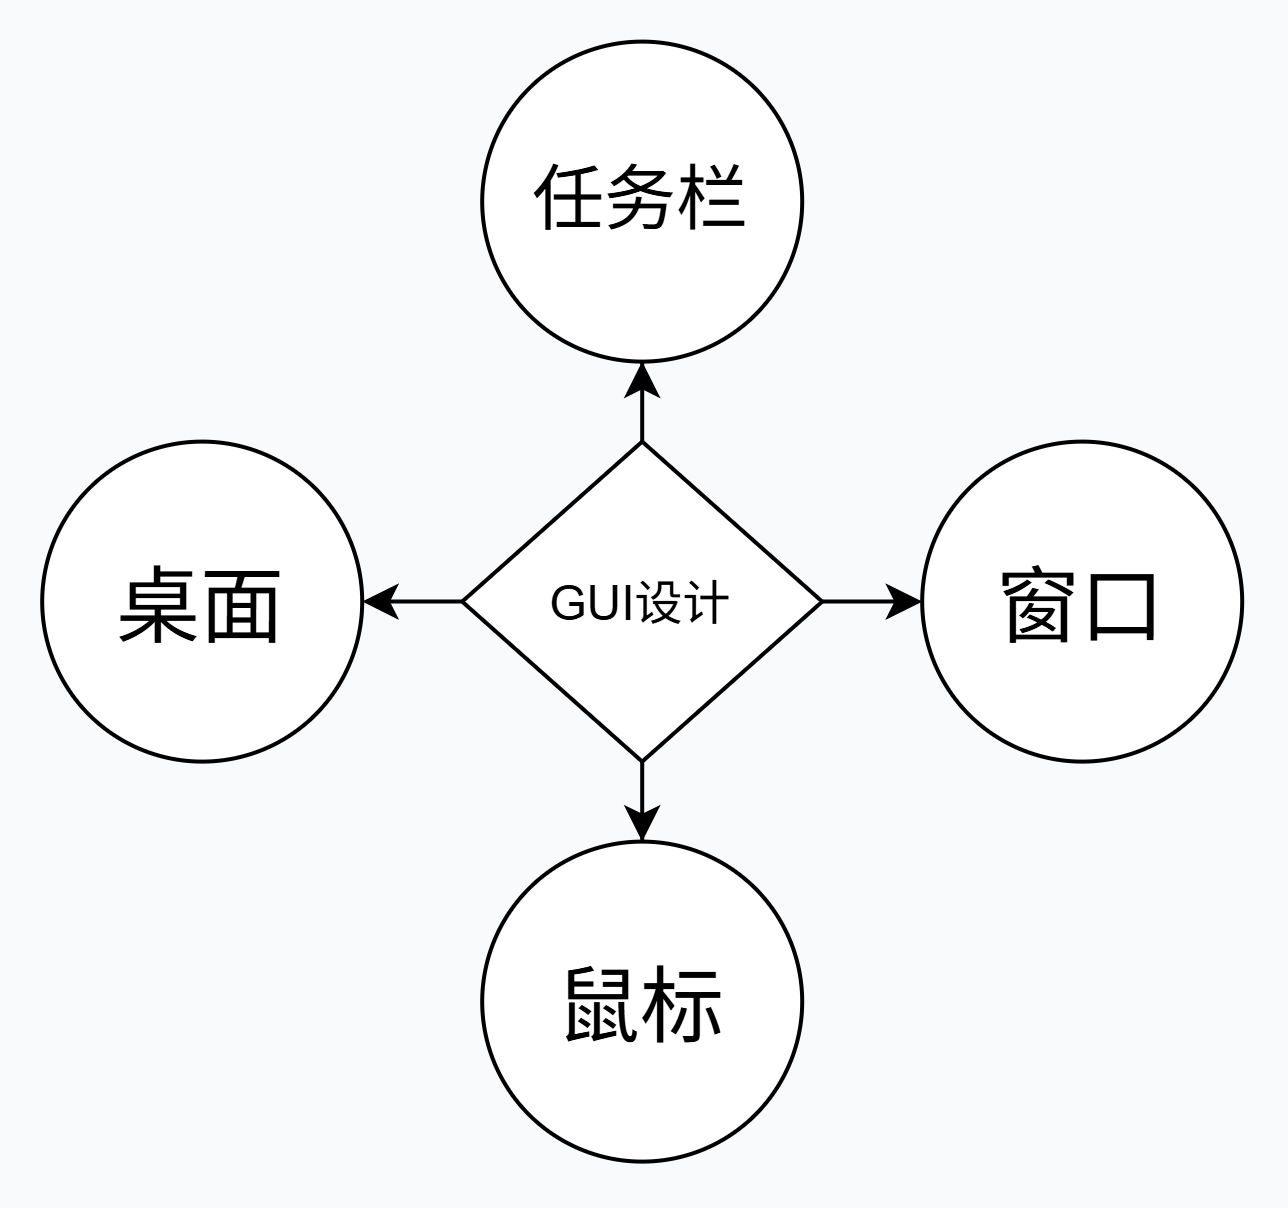
\includegraphics[width=0.5\textwidth]{figure/GUI.png}
  \caption{GUI}
  \label{fig:GUI}
\end{figure}

\begin{figure}[H]
  \centering
  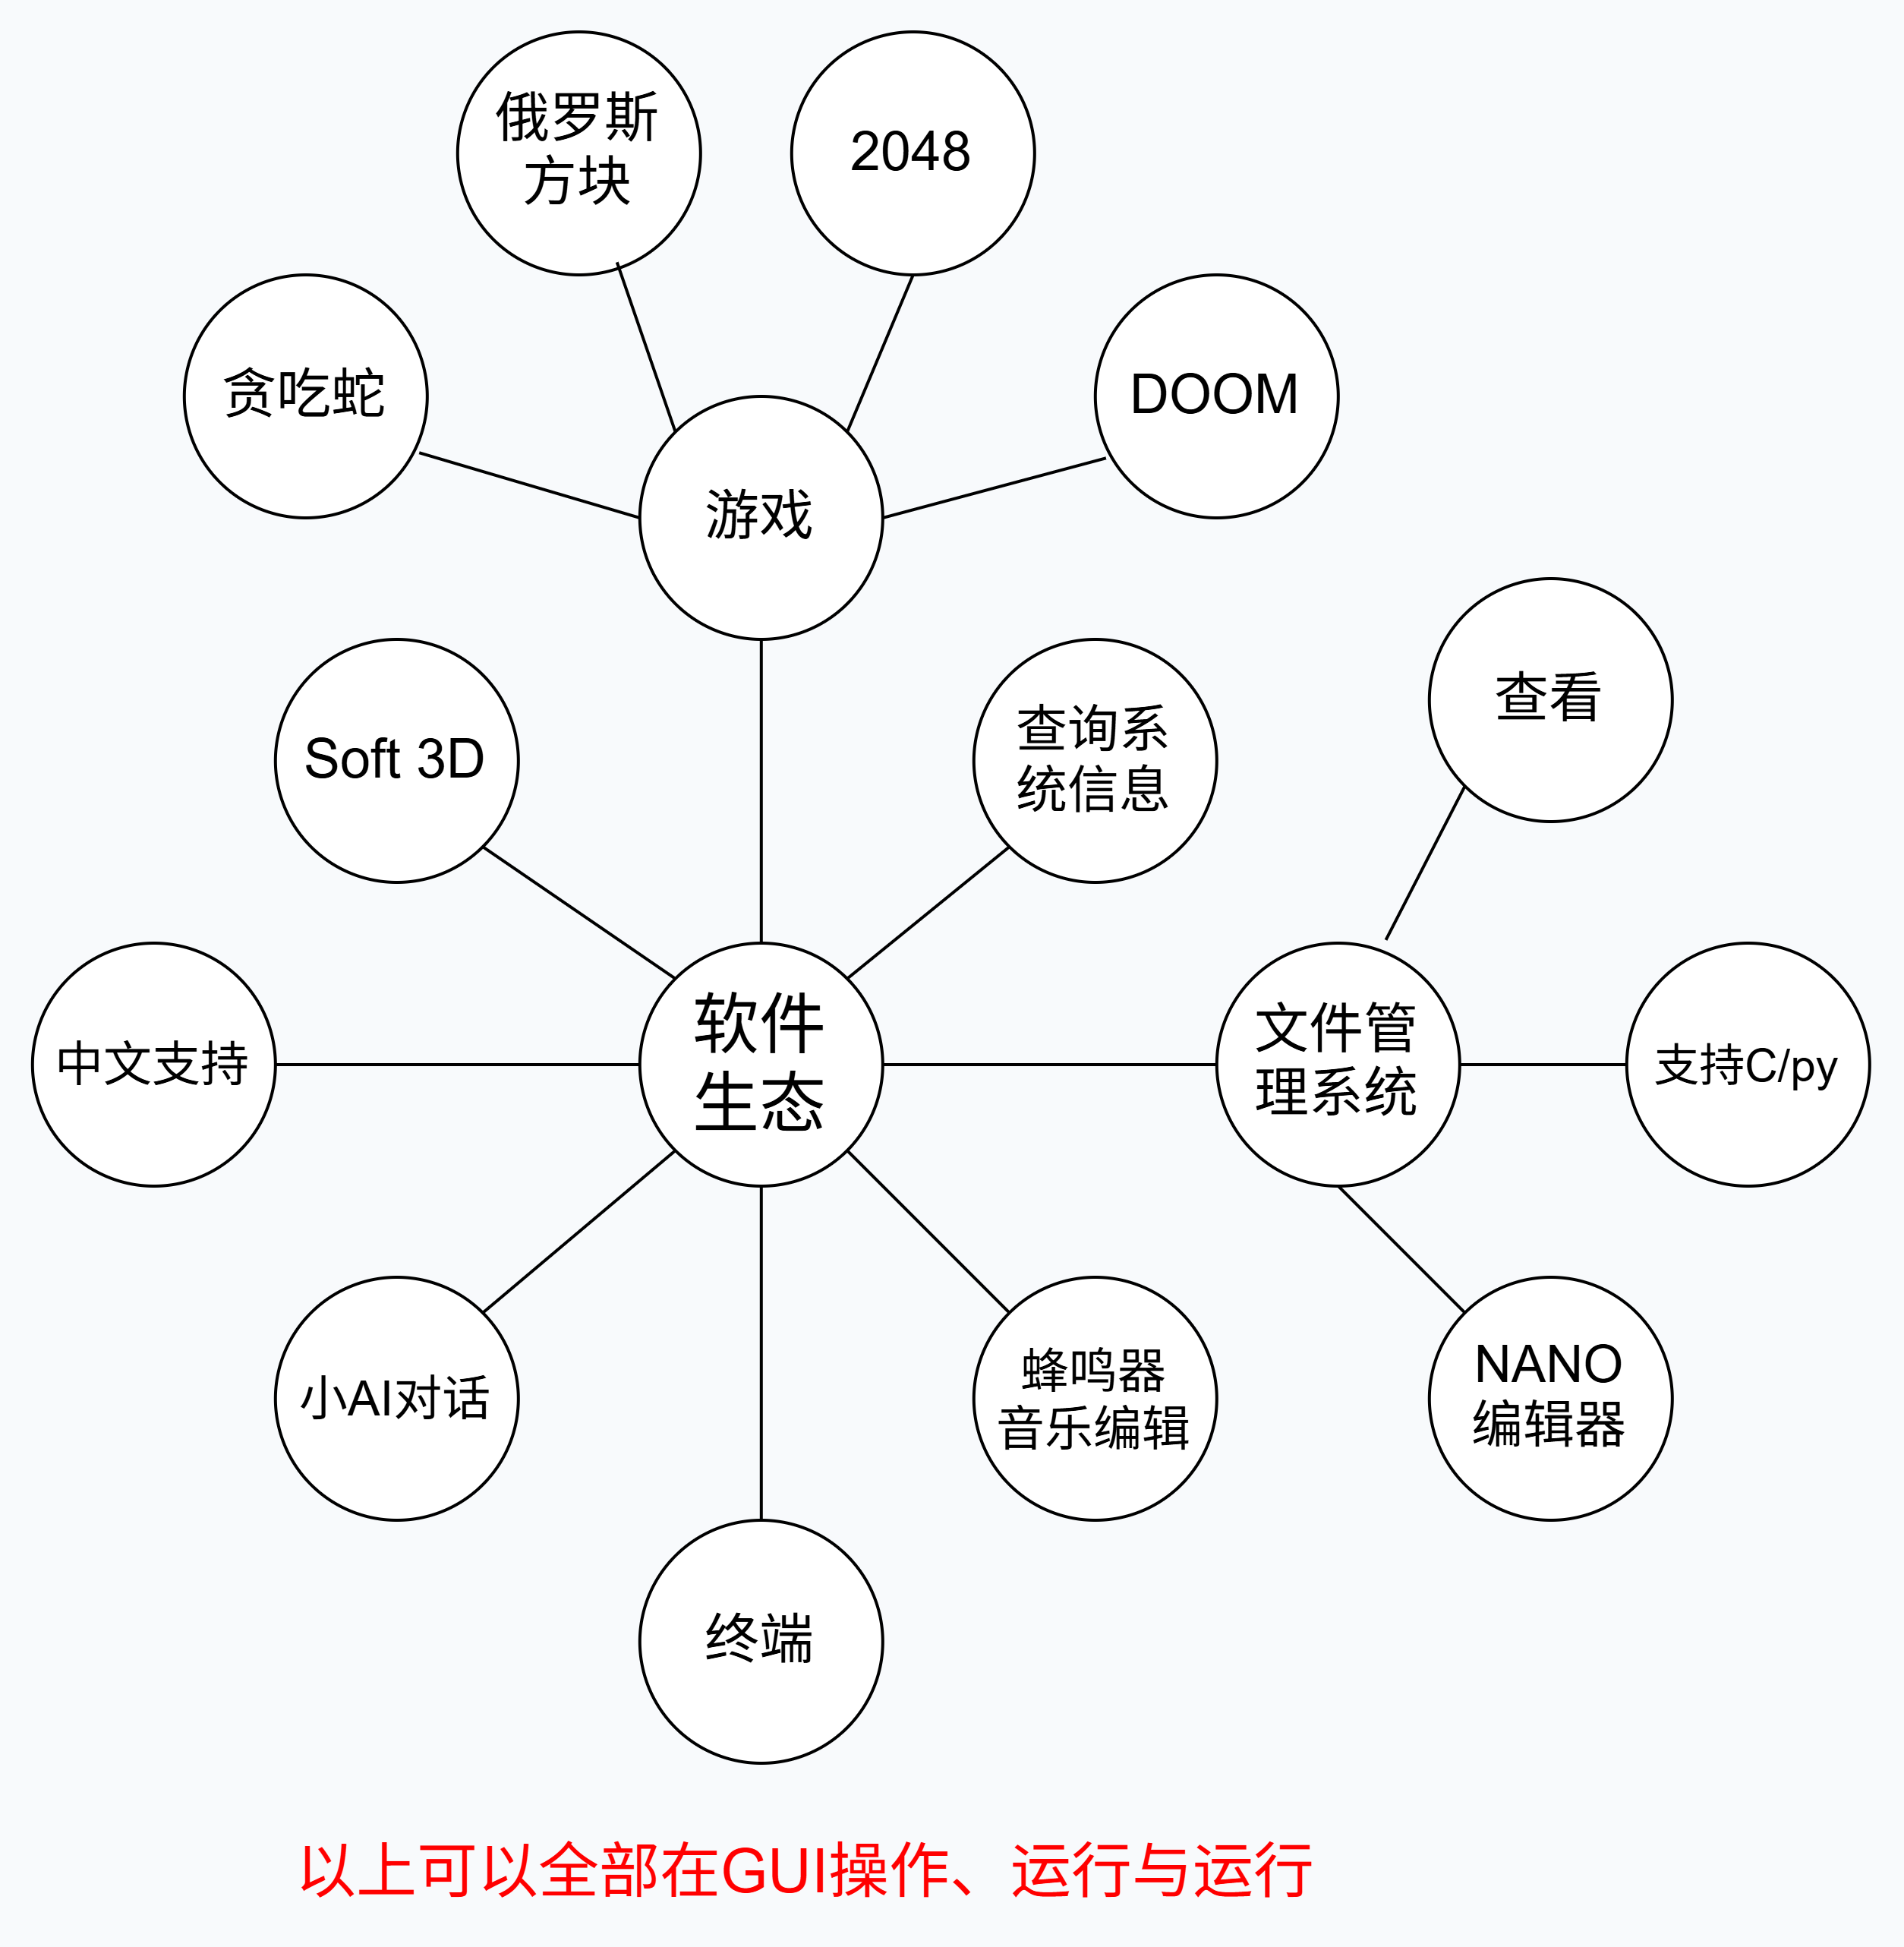
\includegraphics[width=0.95\textwidth]{figure/软件生态.png}
  \caption{软件生态}
  \label{fig:软件生态}
\end{figure}

\subsubsection{GUI展示}

我们的GUI支持完整的桌面、鼠标（ LCD 控制）、任务栏、时间、多窗口、鼠标拖拽等设计。如下：

\begin{figure}[H]
  \centering
  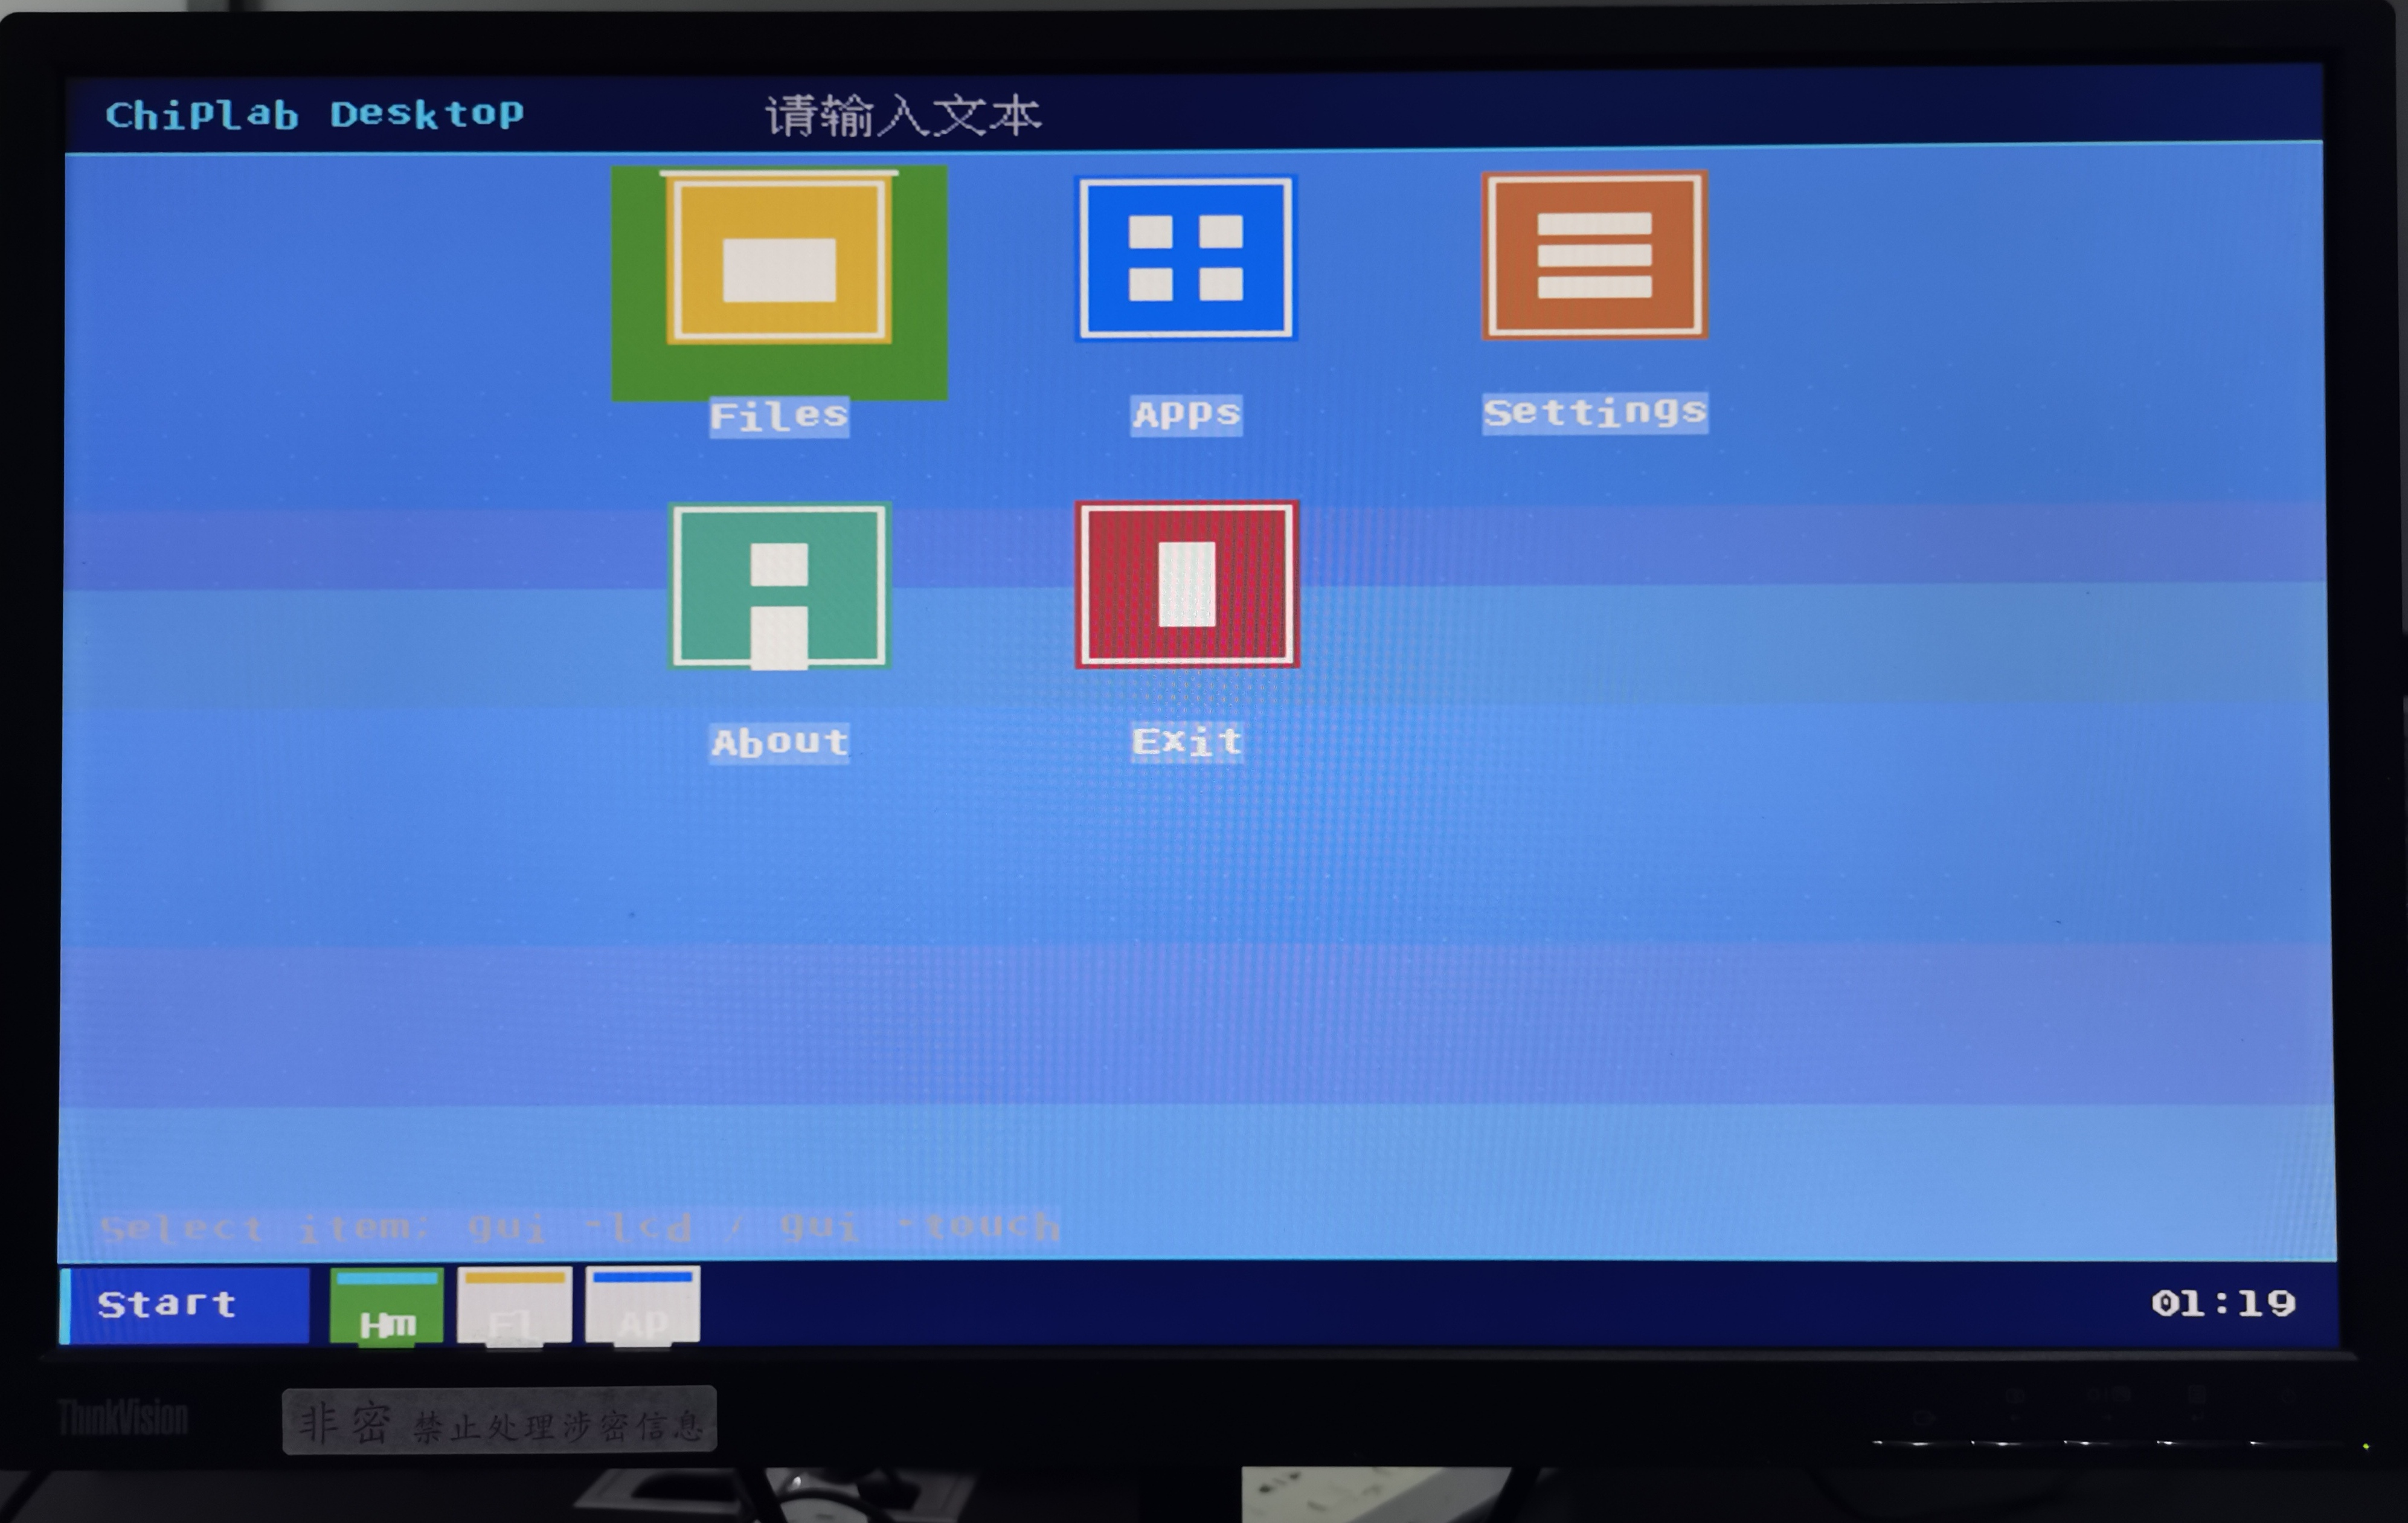
\includegraphics[width=0.95\textwidth]{figure/GUI桌面.jpg}
  \caption{GUI 桌面}
  \label{fig:GUI 桌面}
\end{figure}

\begin{figure}[H]
  \centering
  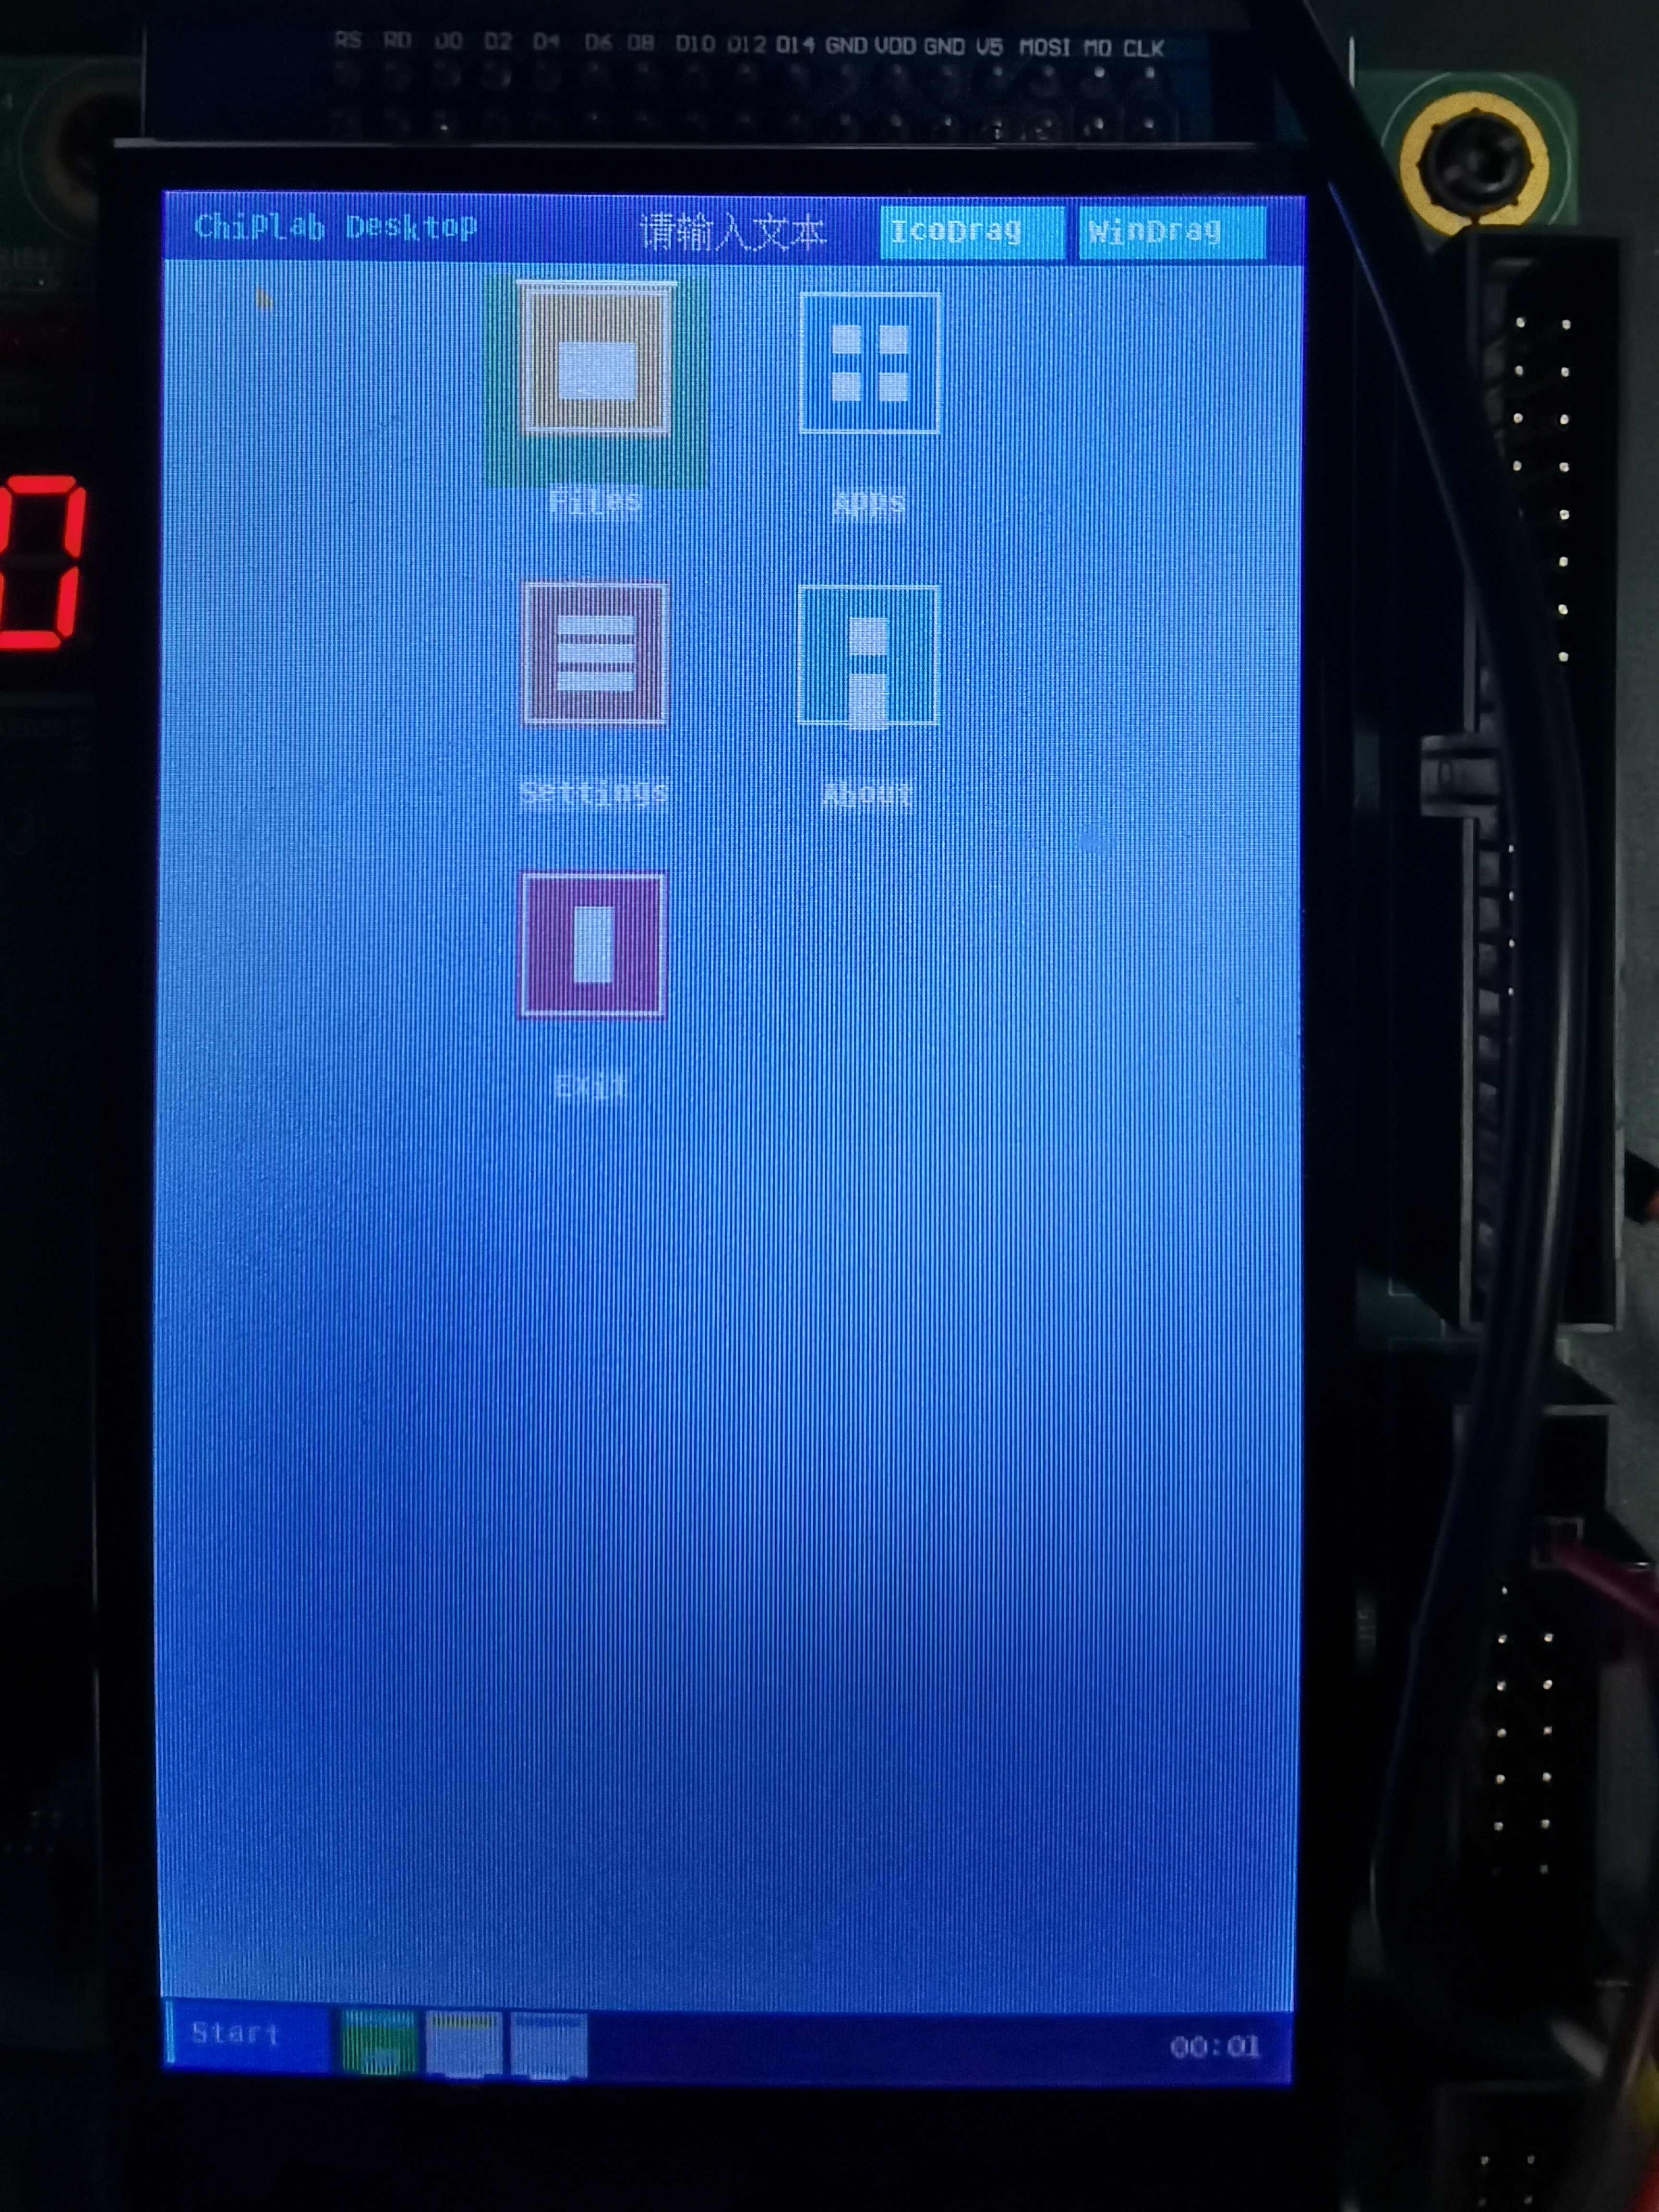
\includegraphics[width=0.3\textwidth]{figure/LCD_GUI.jpg}
  \caption{LCD GUI}
  \label{fig:LCD GUI}
\end{figure}

\begin{figure}[H]
  \centering
  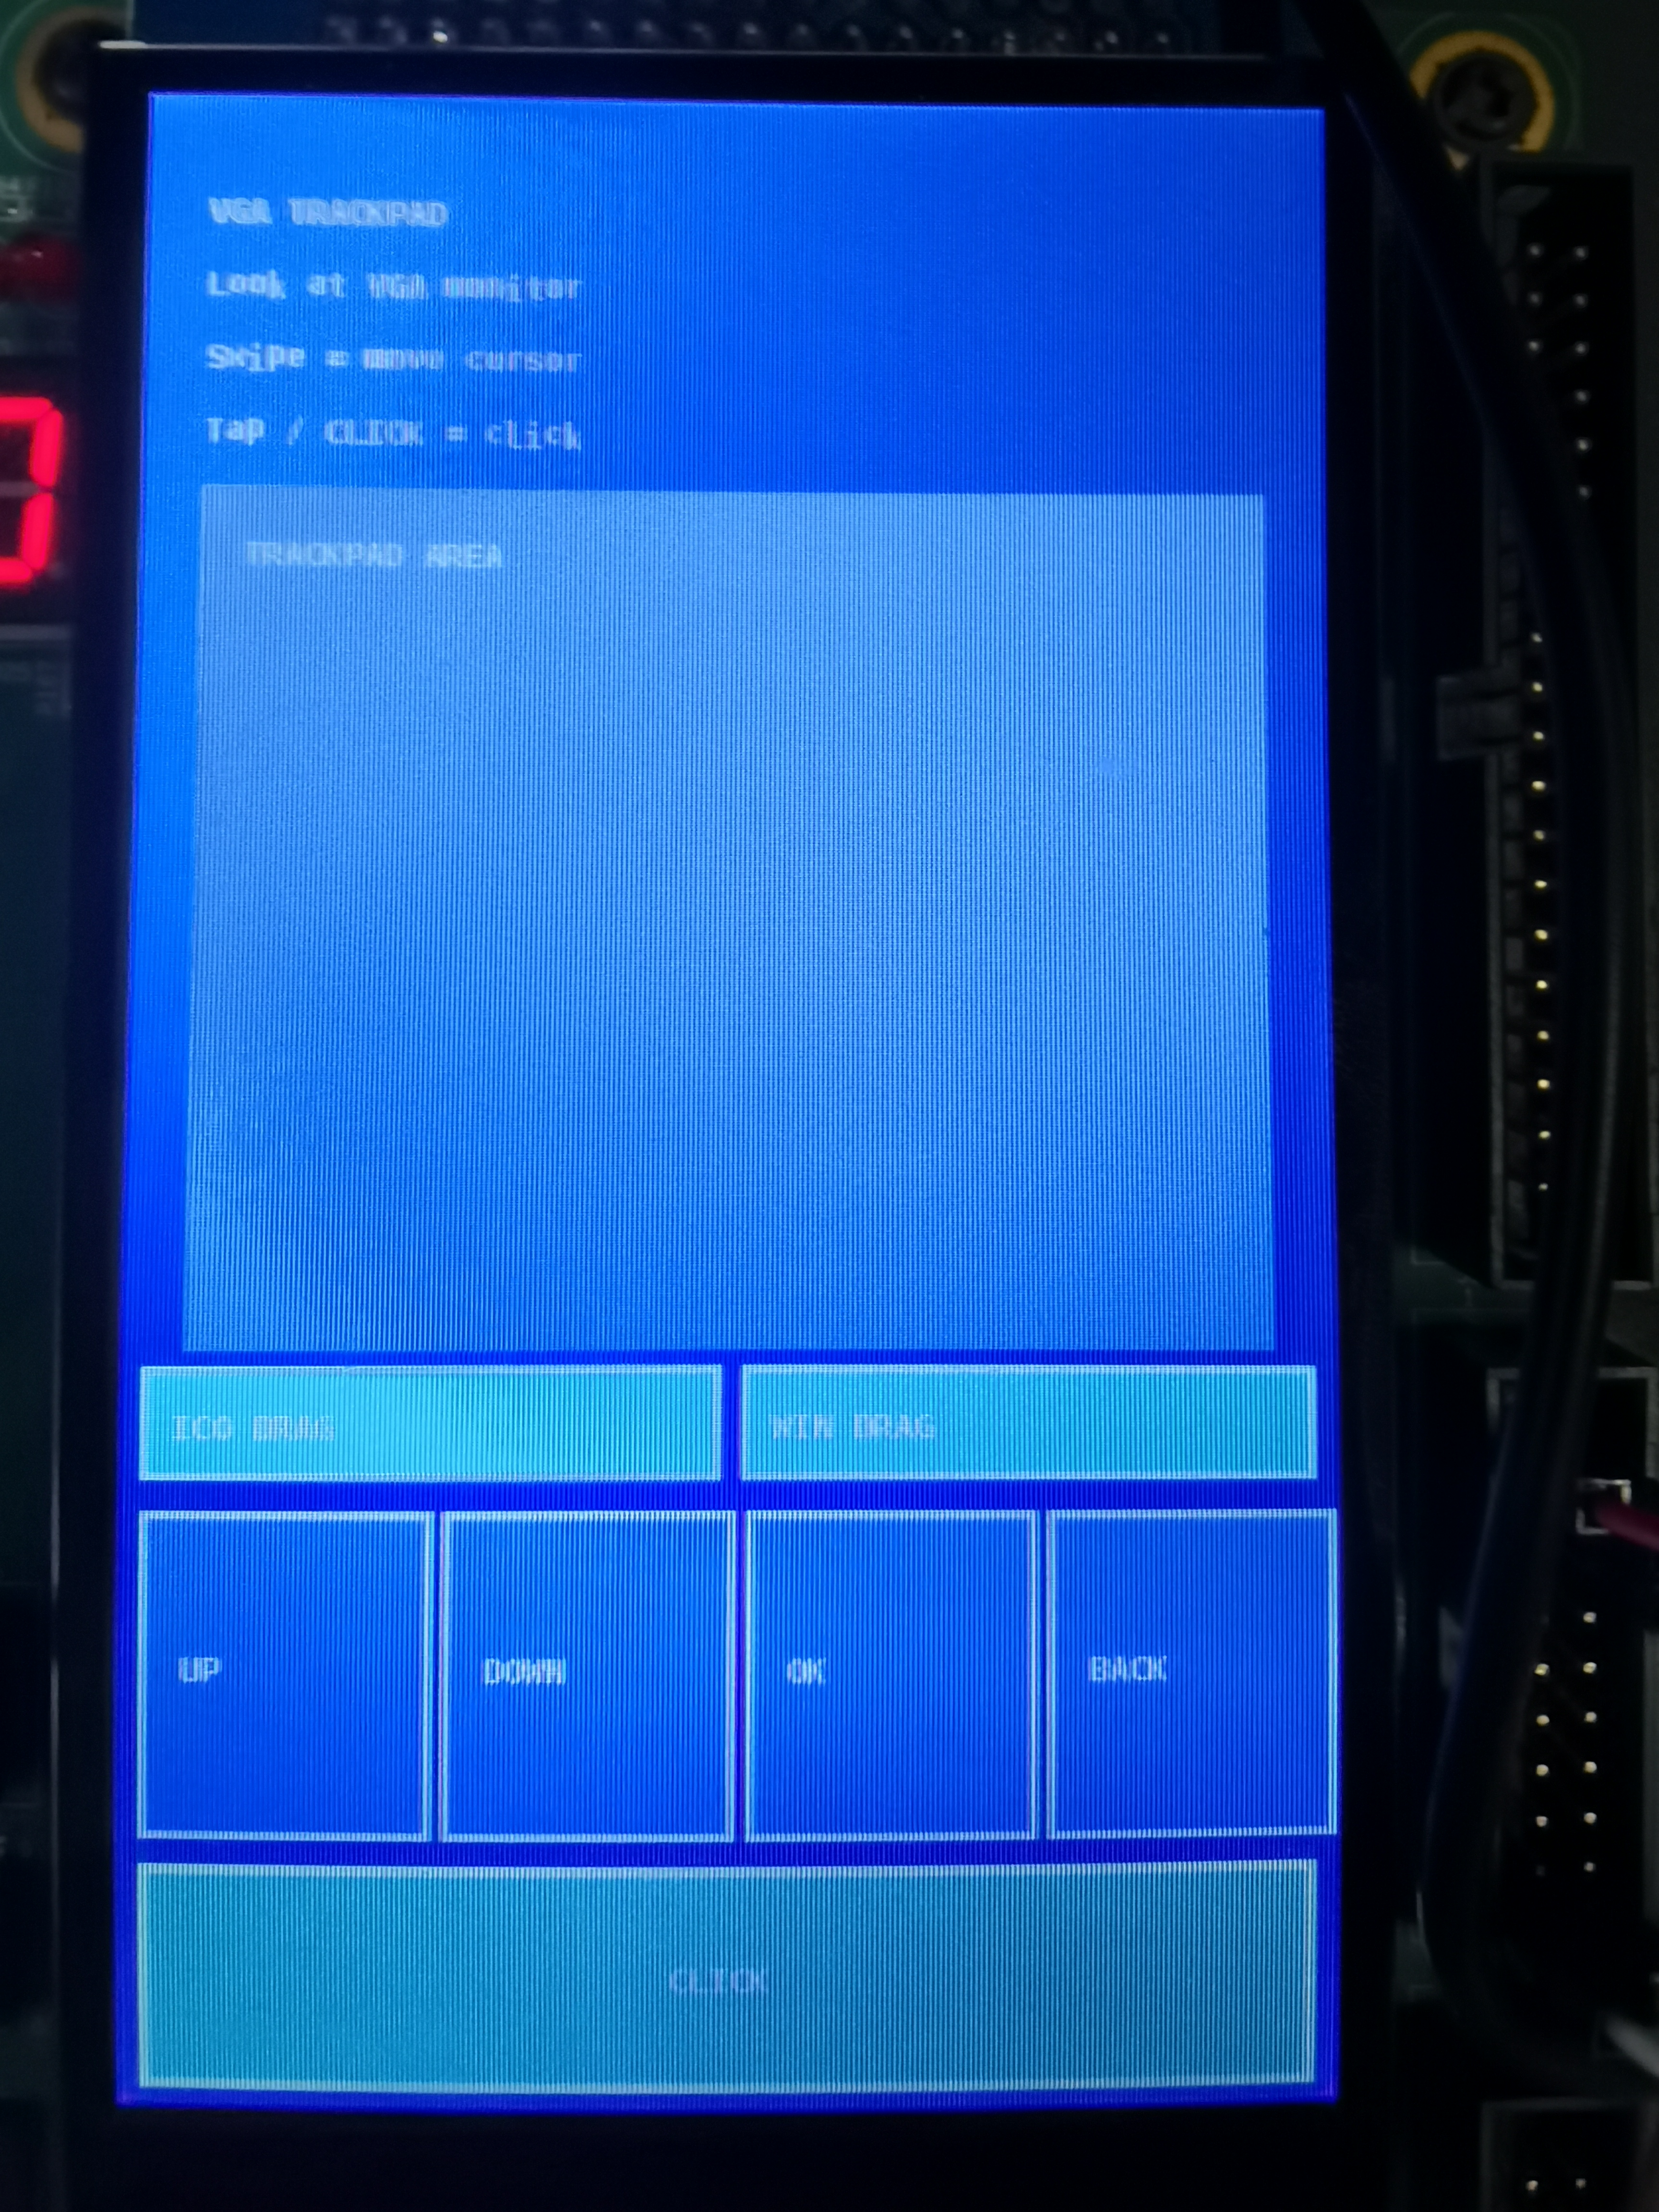
\includegraphics[width=0.3\textwidth]{figure/LCD_Mouse.jpg}
  \caption{LCD Mouse}
  \label{fig:LCD Mouse}
\end{figure}

\begin{figure}[H]
  \centering
  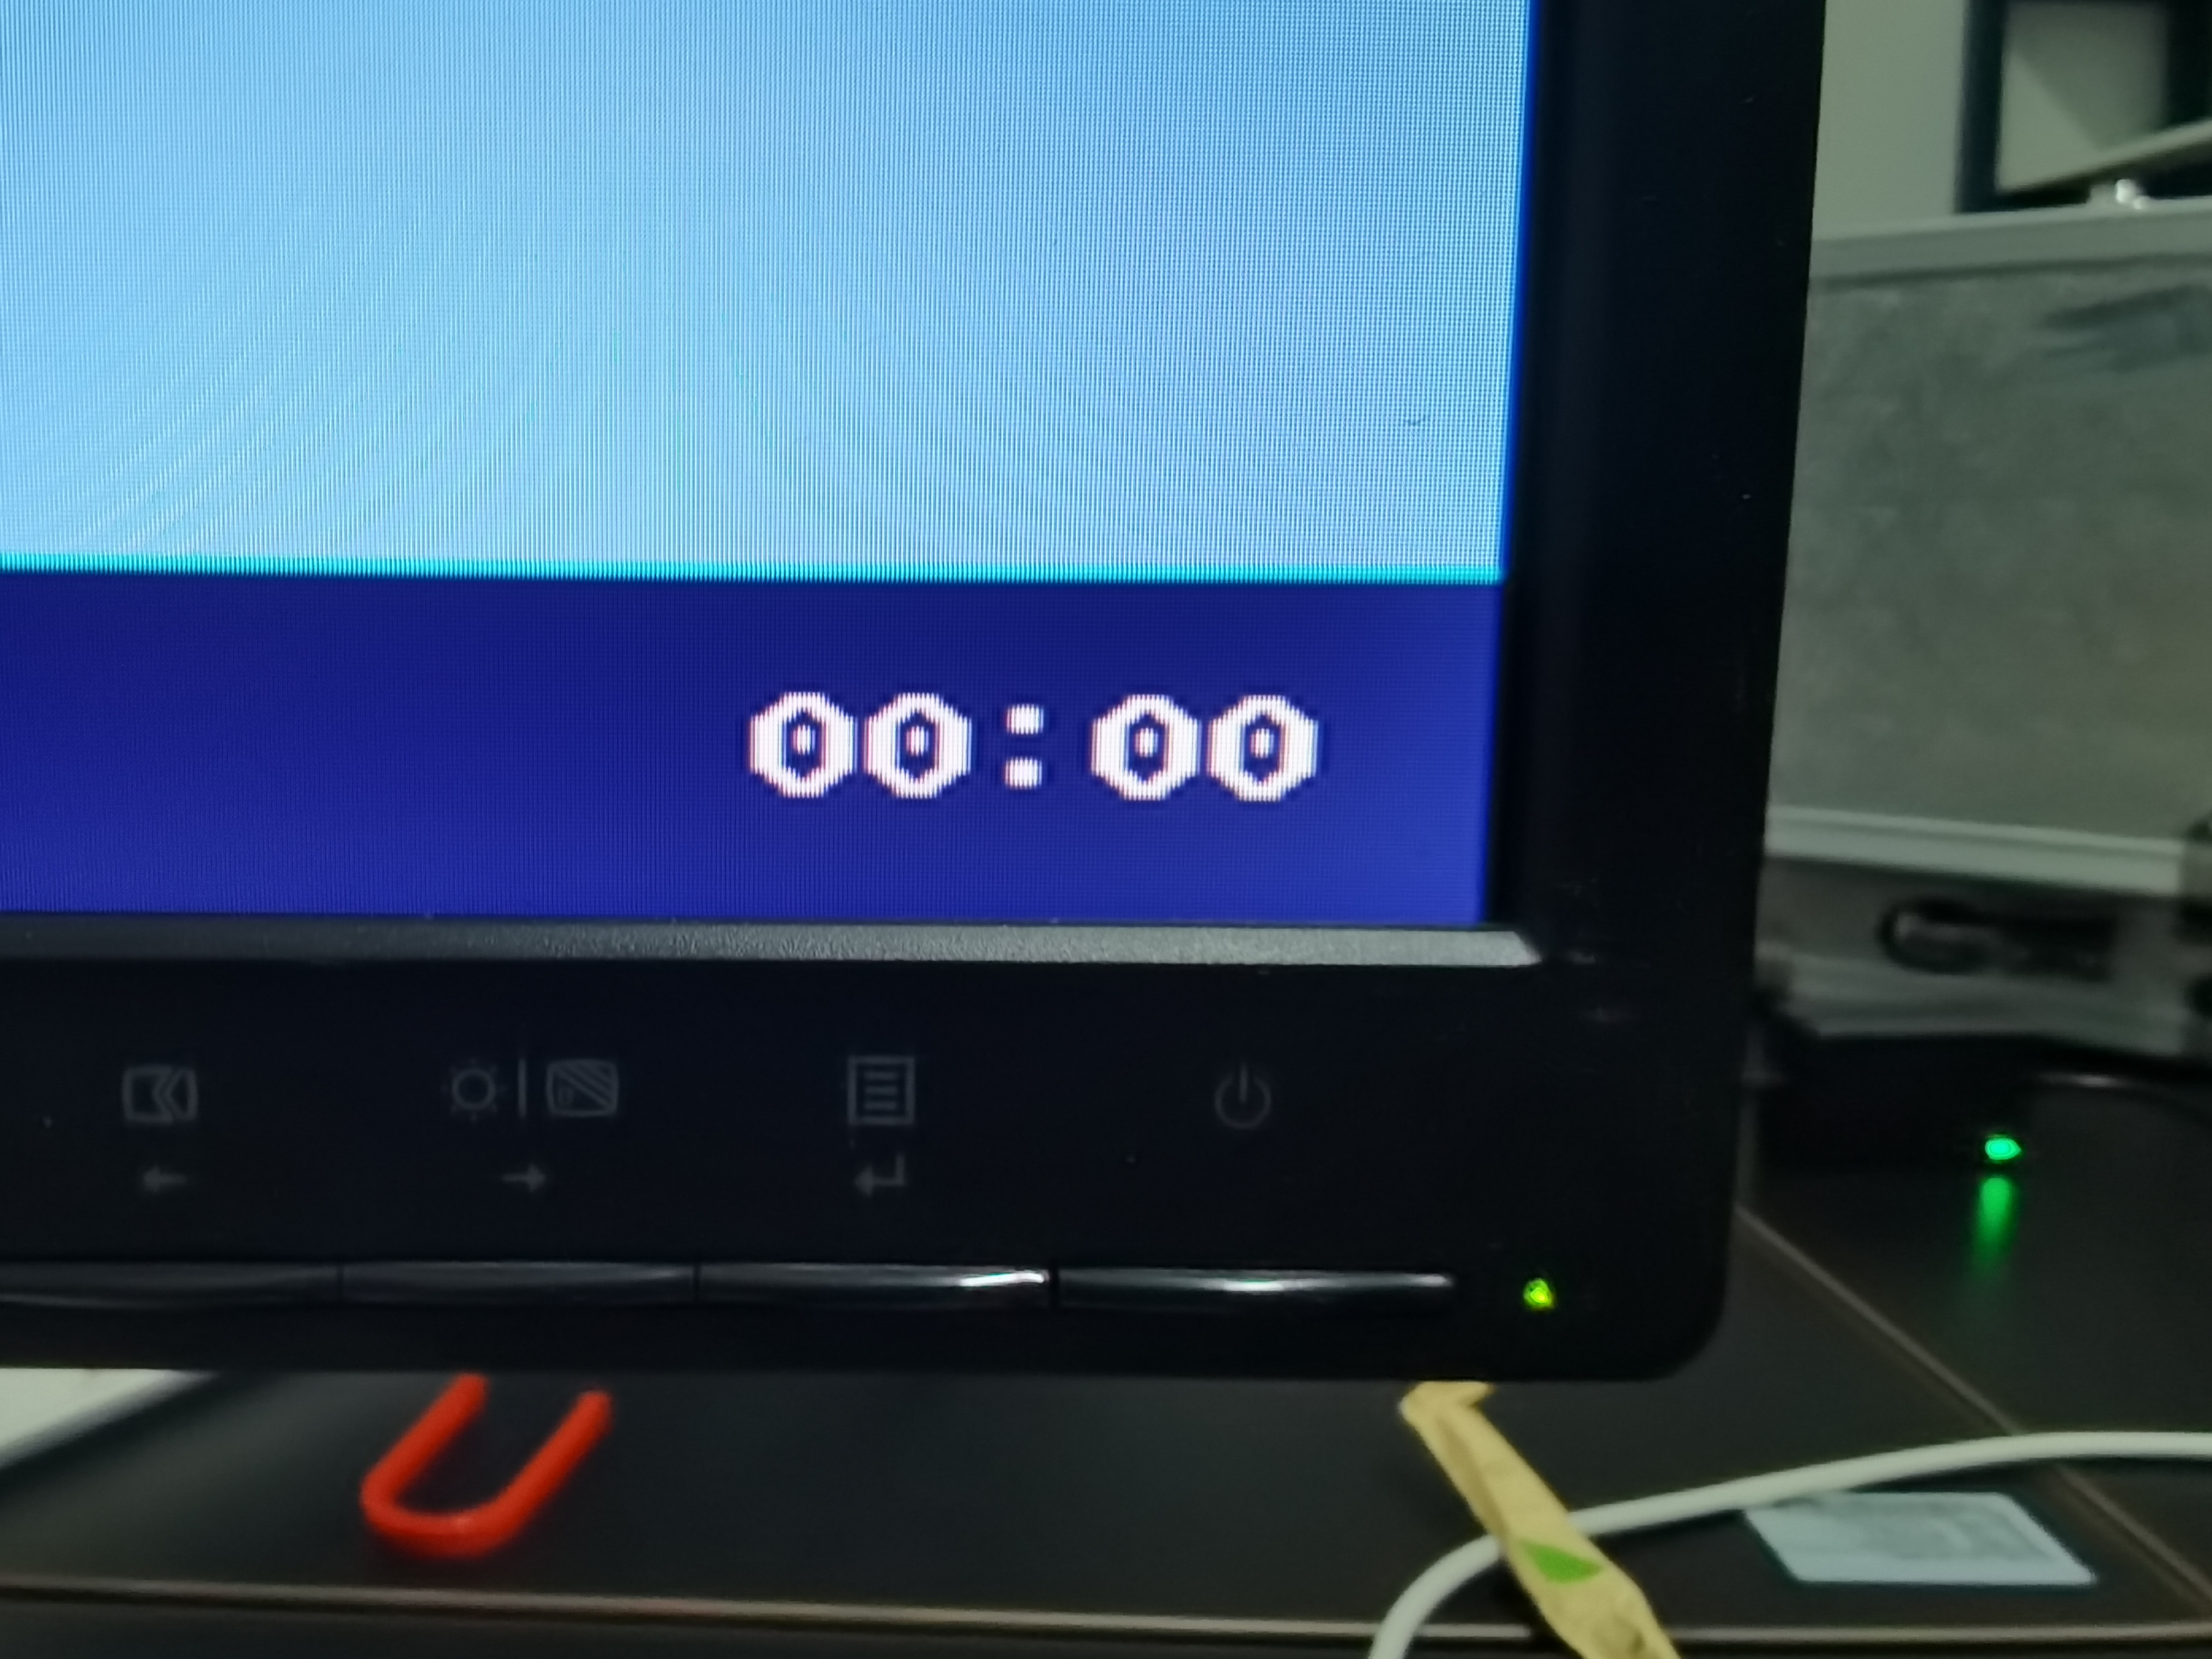
\includegraphics[width=0.3\textwidth]{figure/LCD_Time.jpg}
  \caption{LCD Time}
  \label{fig:LCD Time}
\end{figure}

\begin{figure}[H]
  \centering
  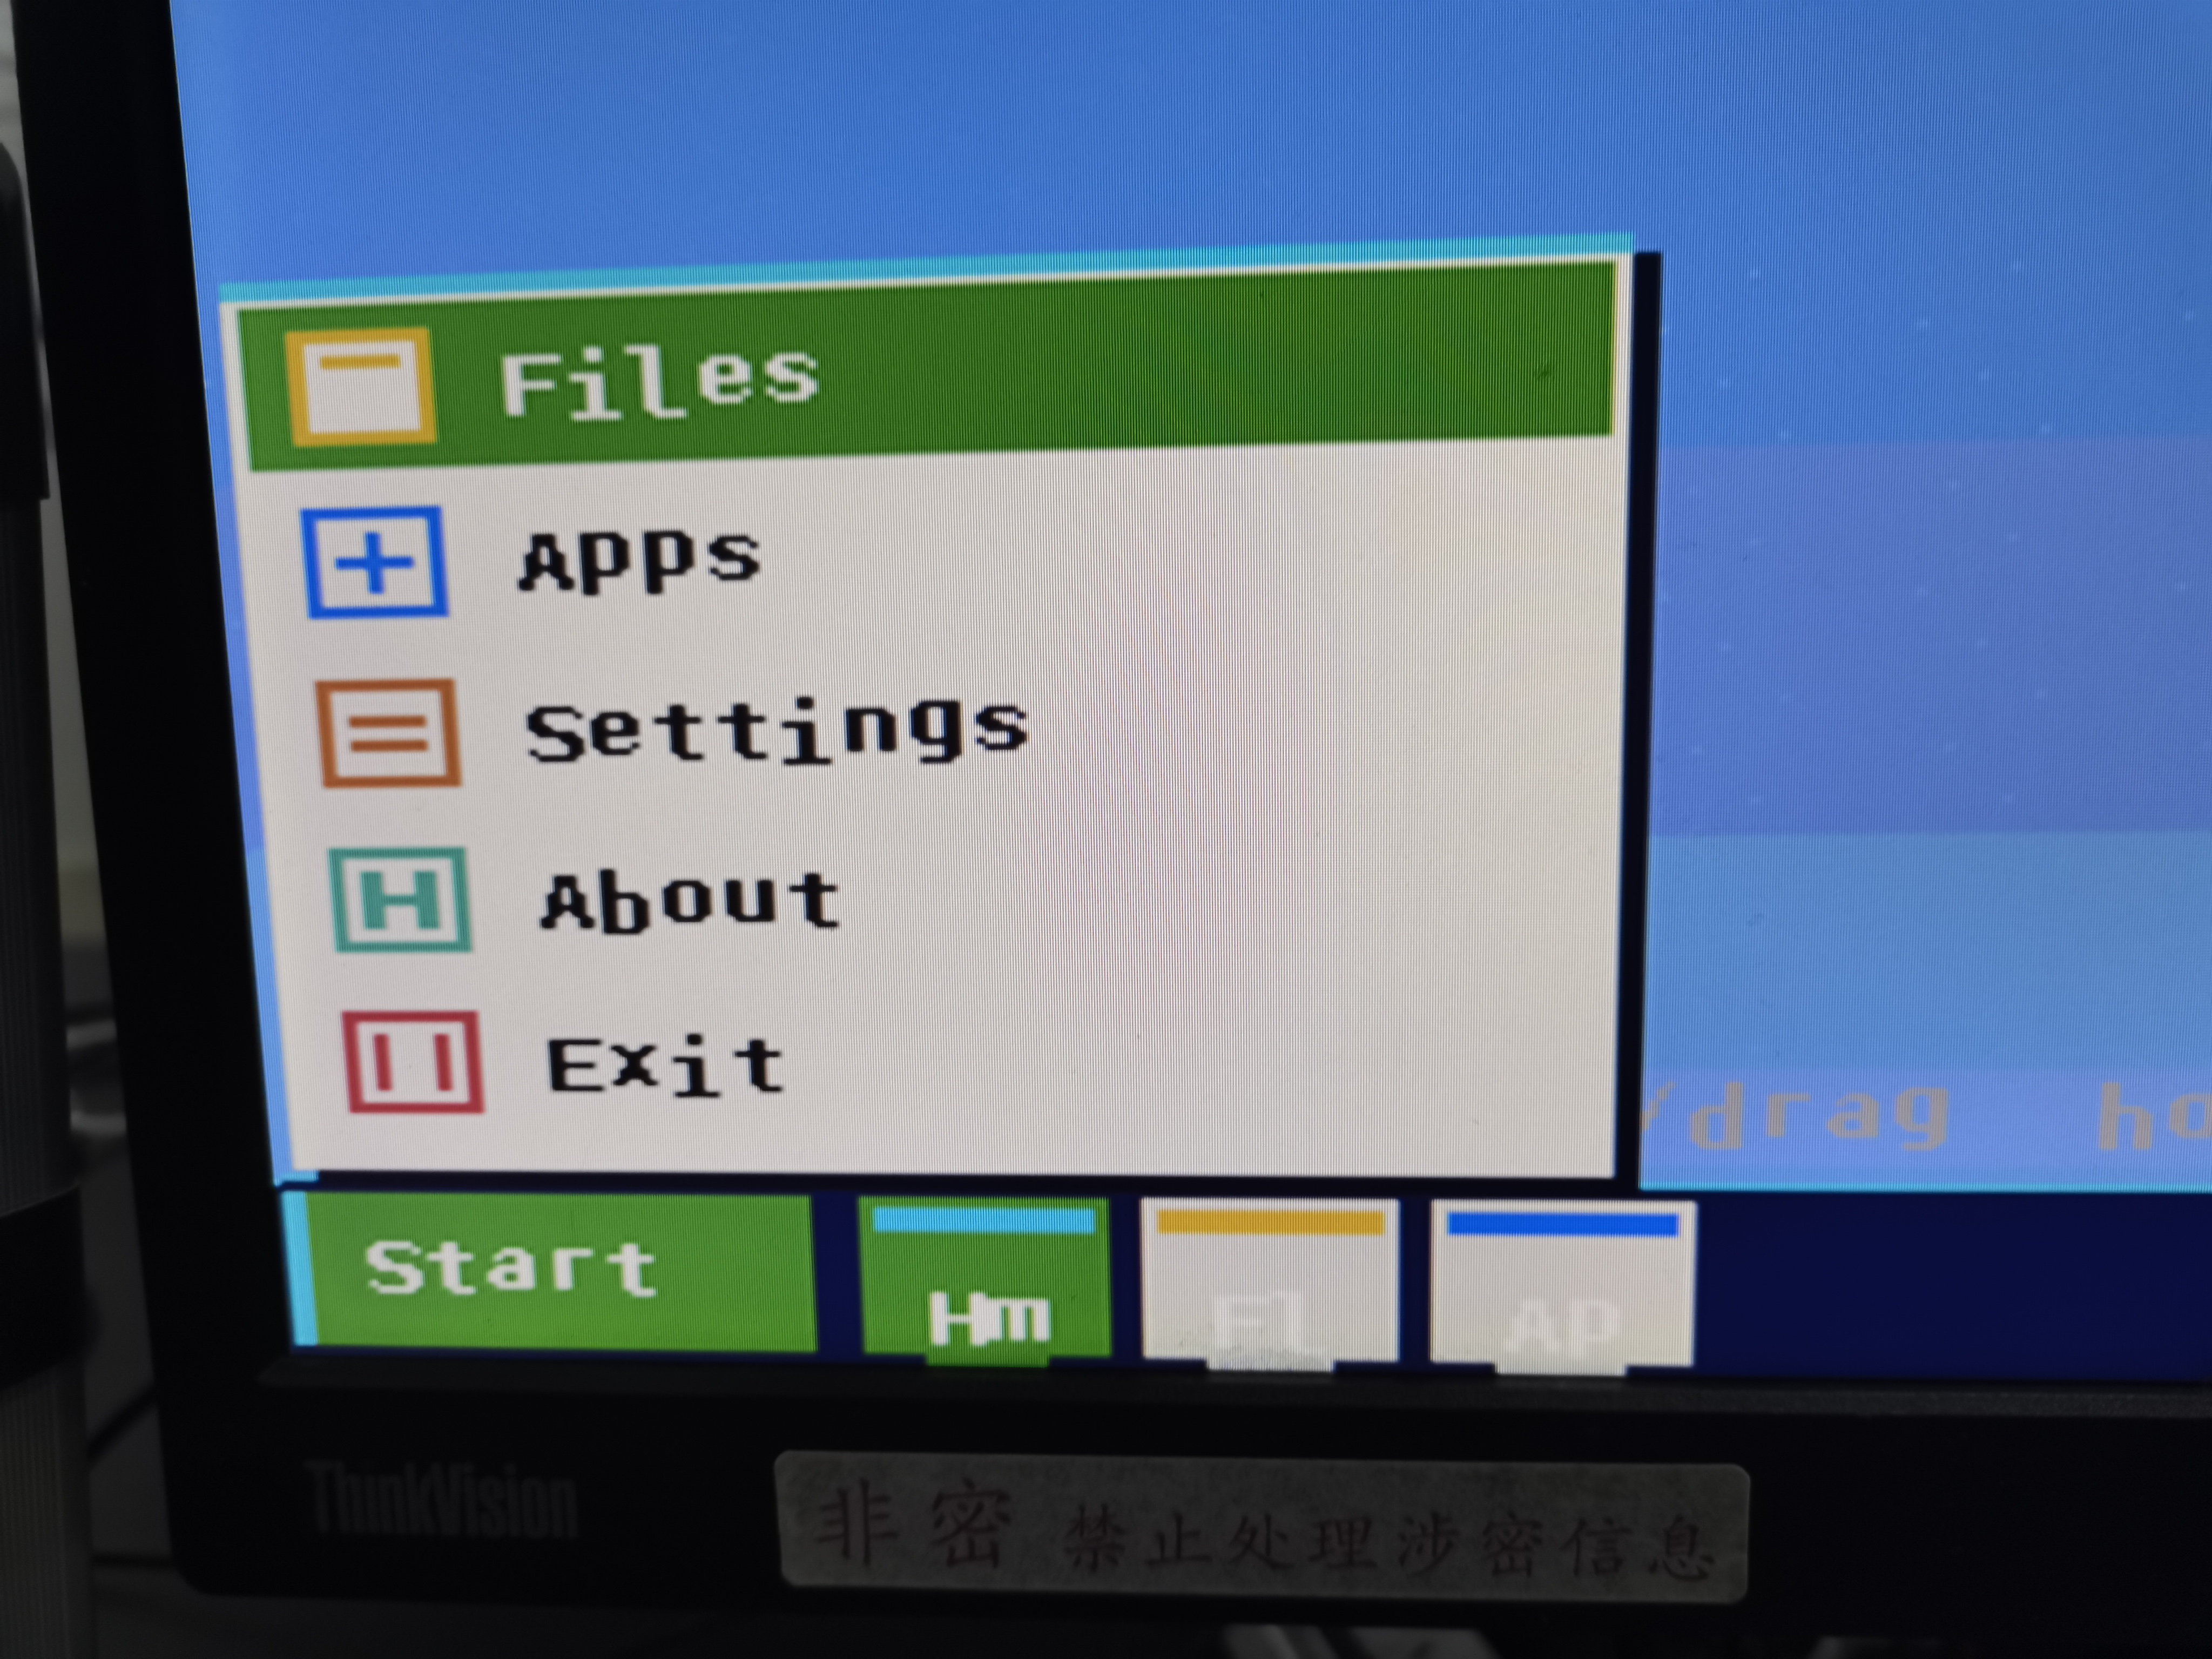
\includegraphics[width=0.3\textwidth]{figure/菜单栏.jpg}
  \caption{菜单栏}
  \label{fig:菜单栏}
\end{figure}

\begin{figure}[H]
  \centering
  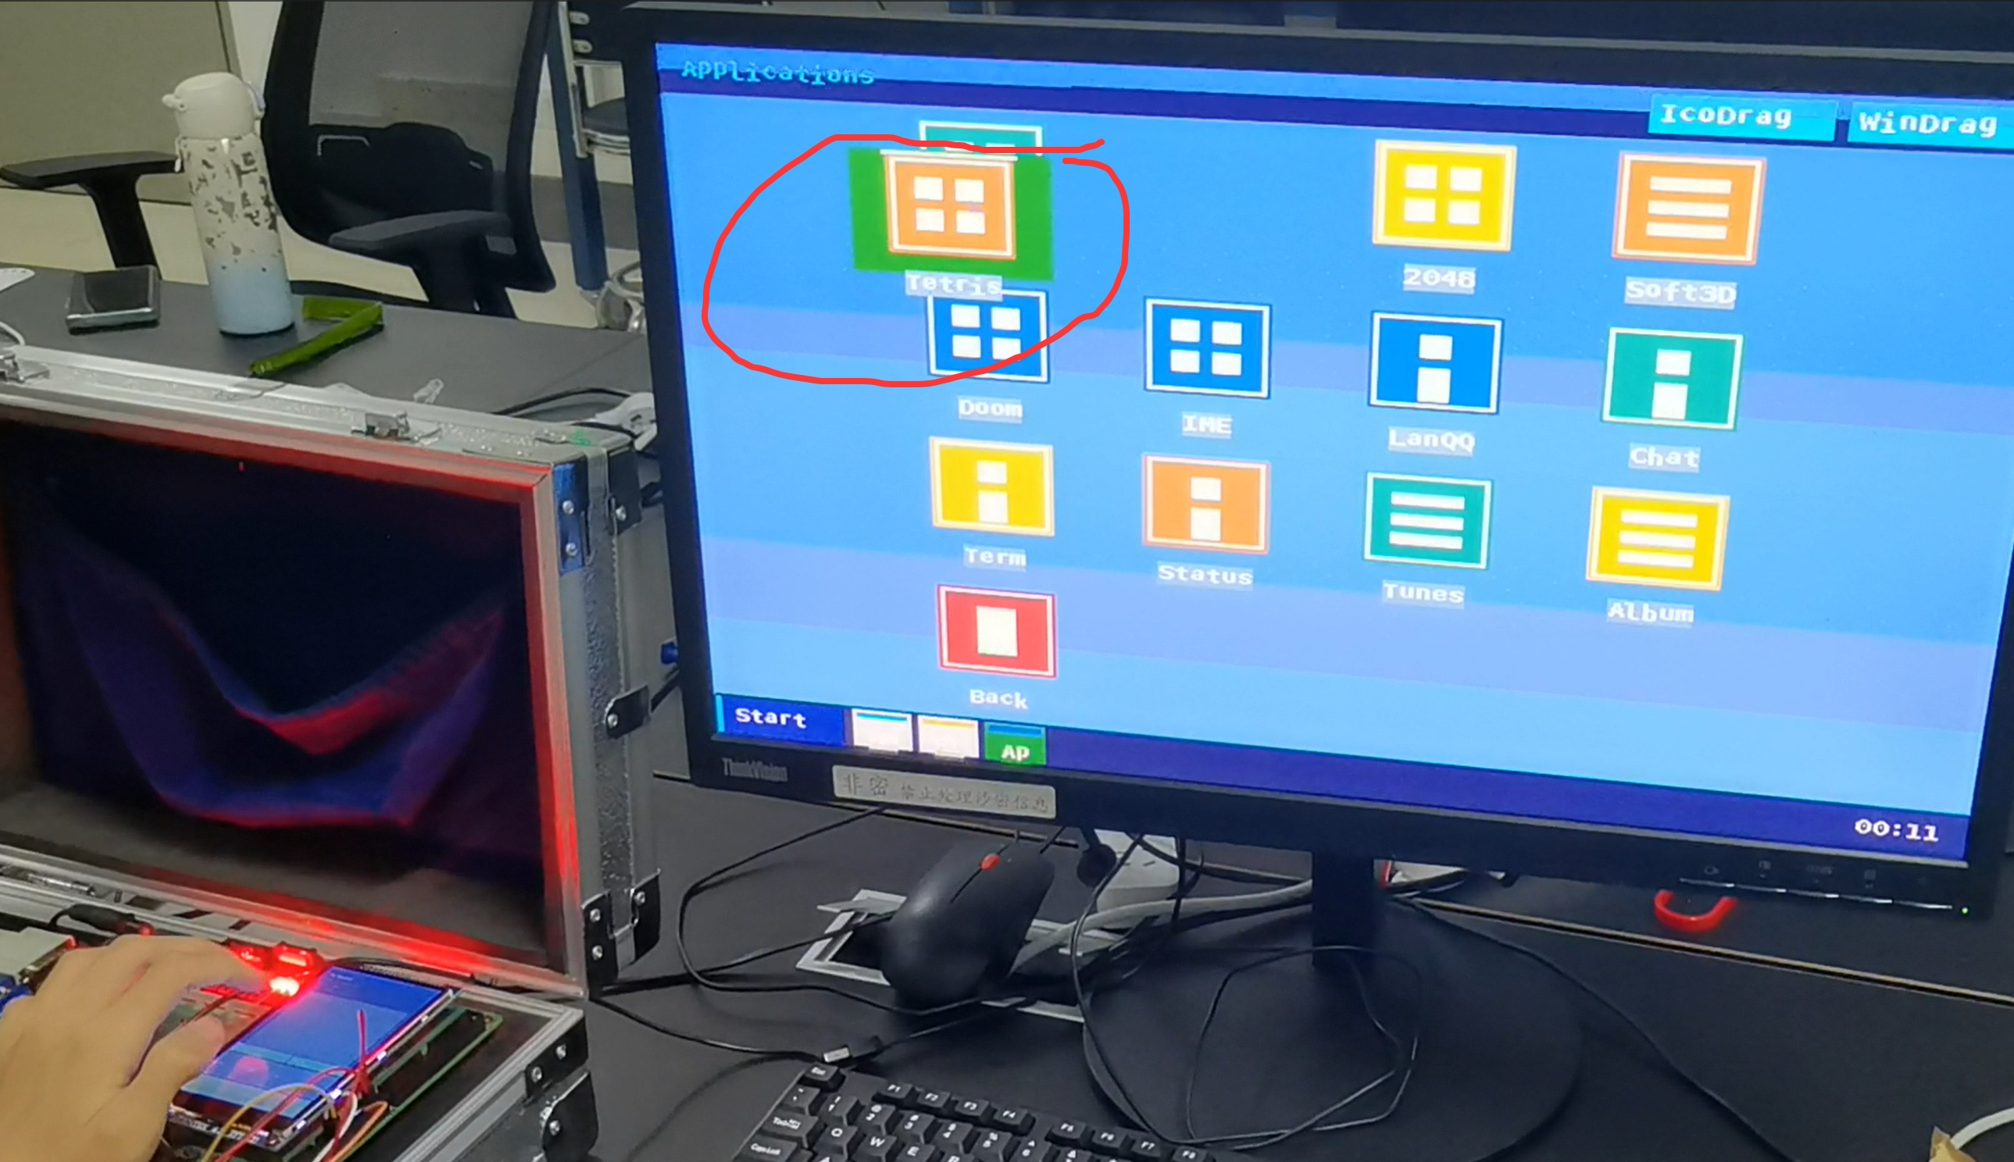
\includegraphics[width=0.95\textwidth]{figure/鼠标拖拽.png}
  \caption{鼠标拖拽}
  \label{fig:鼠标拖拽}
\end{figure}

\subsubsection{软件生态}

我们的 linux 系统支持多种游戏（包括 DOOM）、软浮点 3D 渲染、中文支持、小型意图推理模型、 NANO 编辑、 C/py 编译等。

\begin{figure}[H]
  \centering
  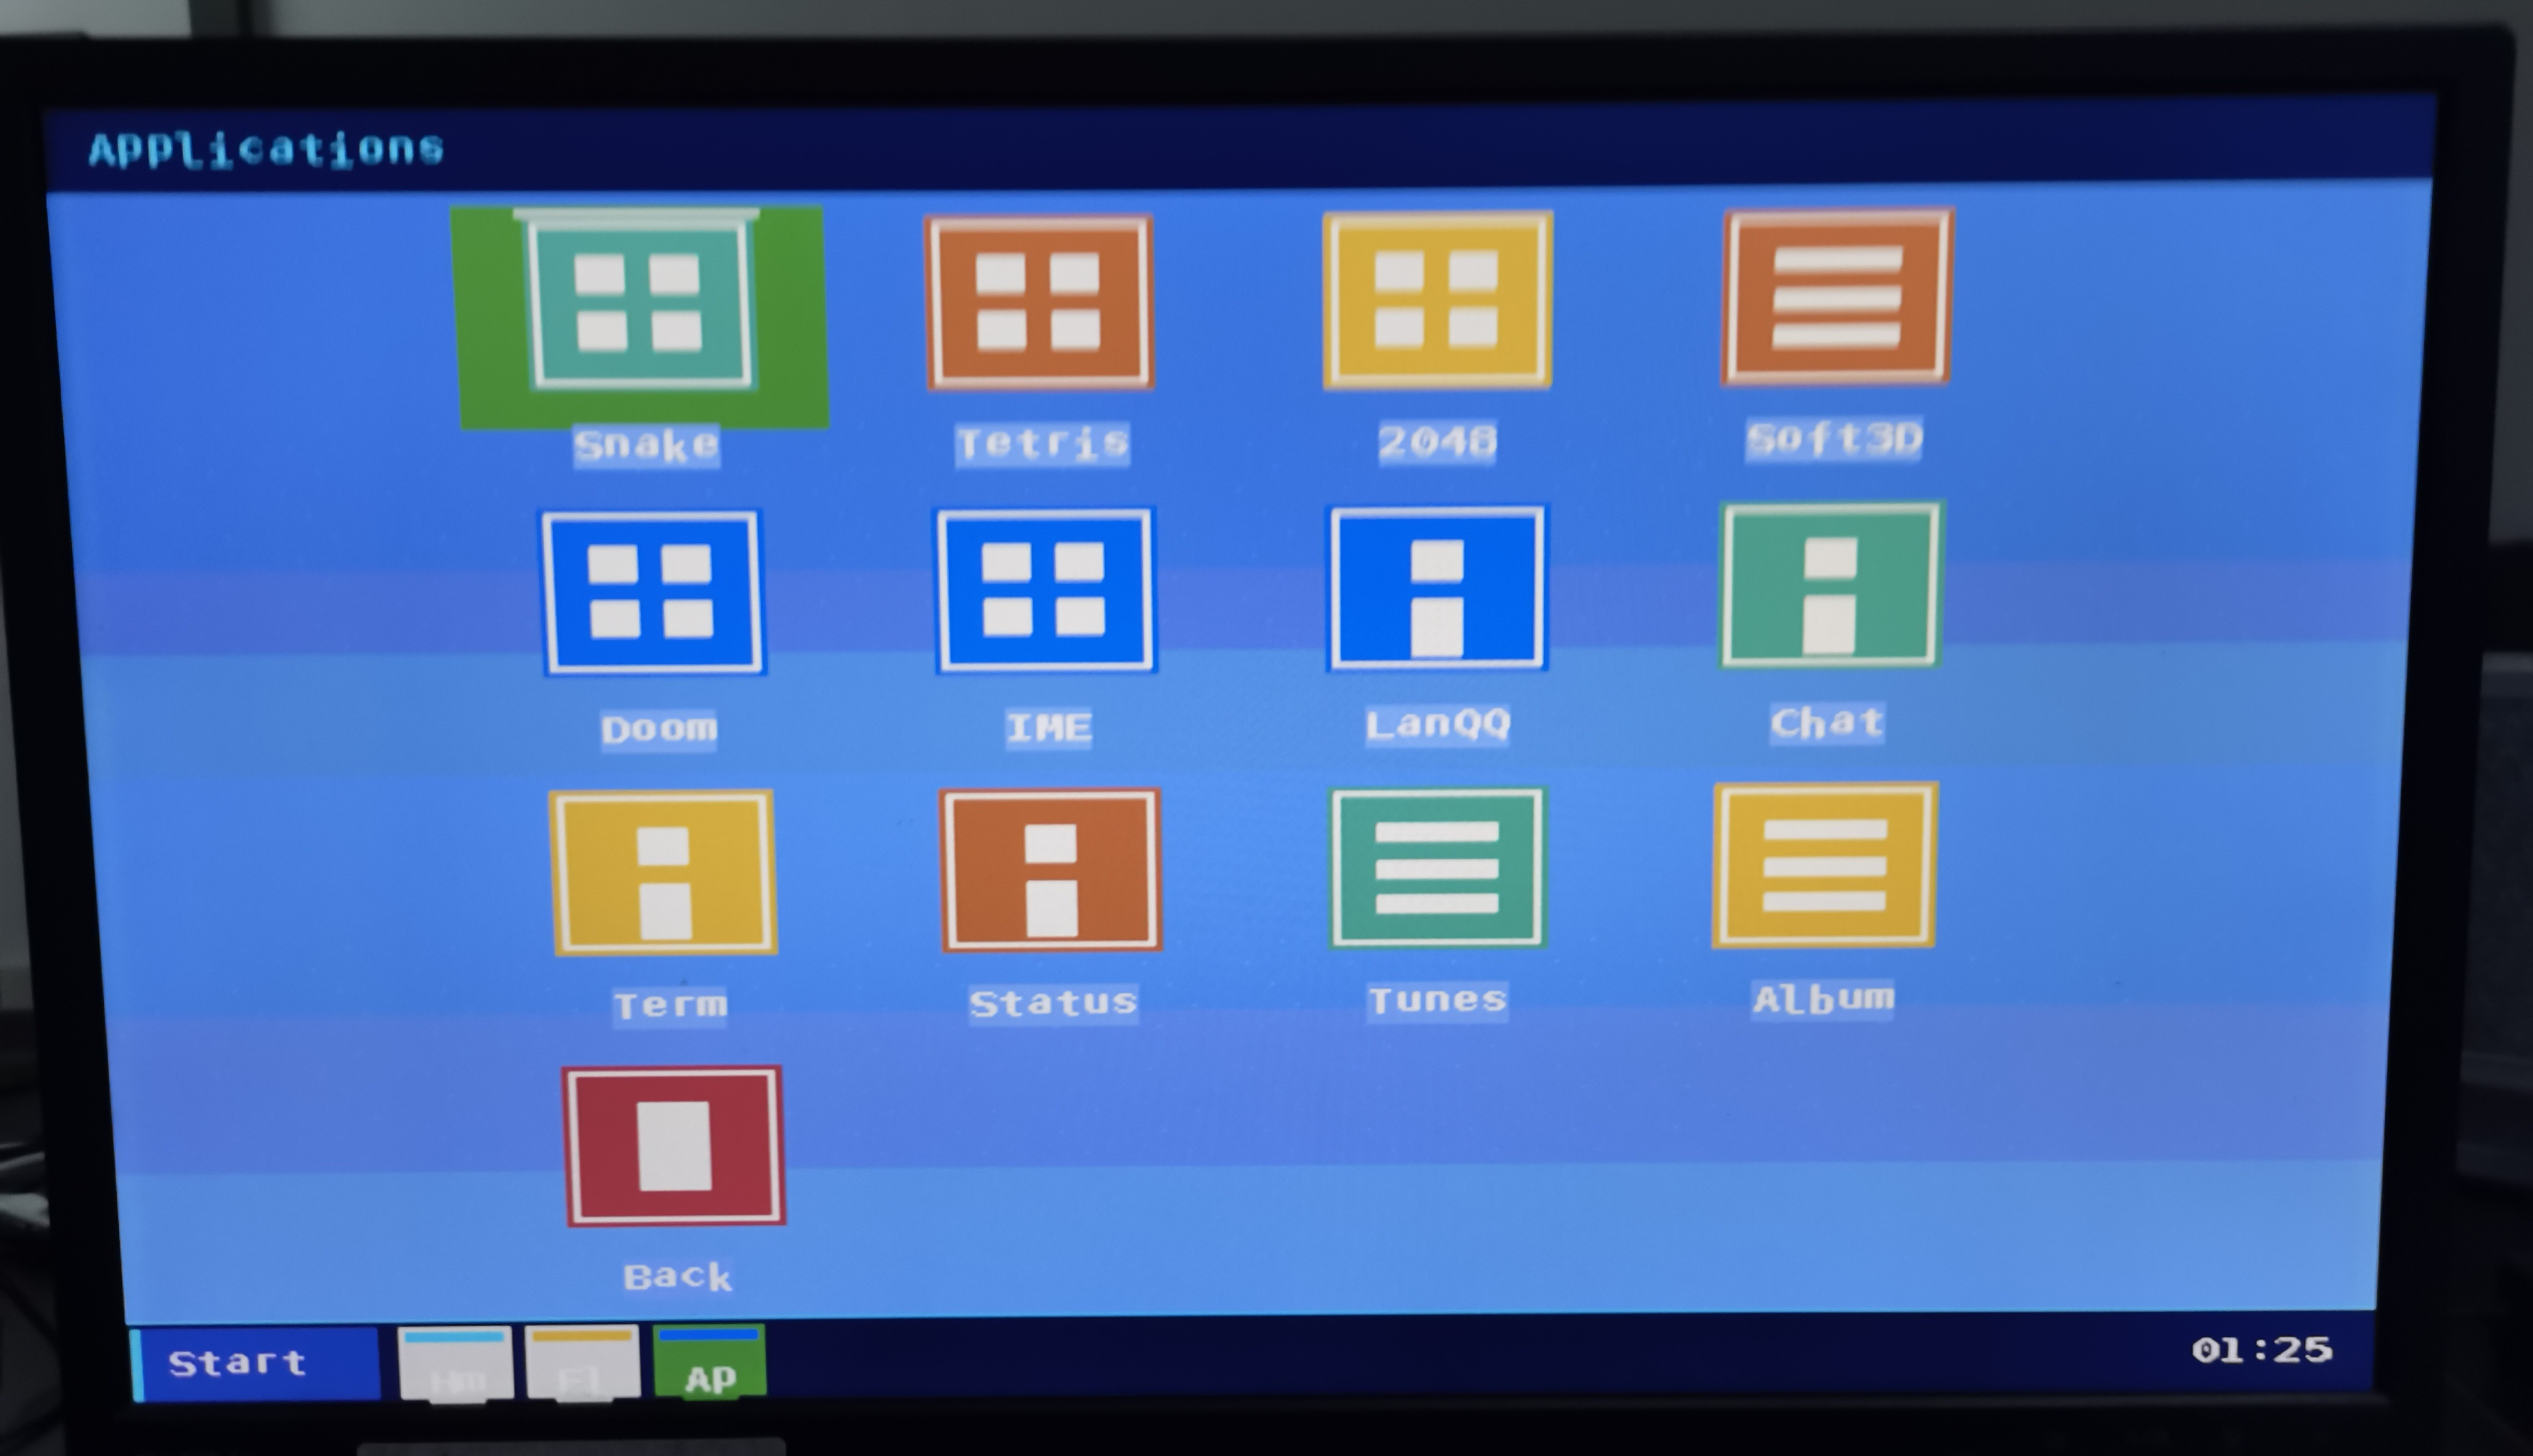
\includegraphics[width=0.95\textwidth]{figure/应用总览.jpg}
  \caption{应用总览}
  \label{fig:应用总览}
\end{figure}

\begin{figure}[H]
  \centering
  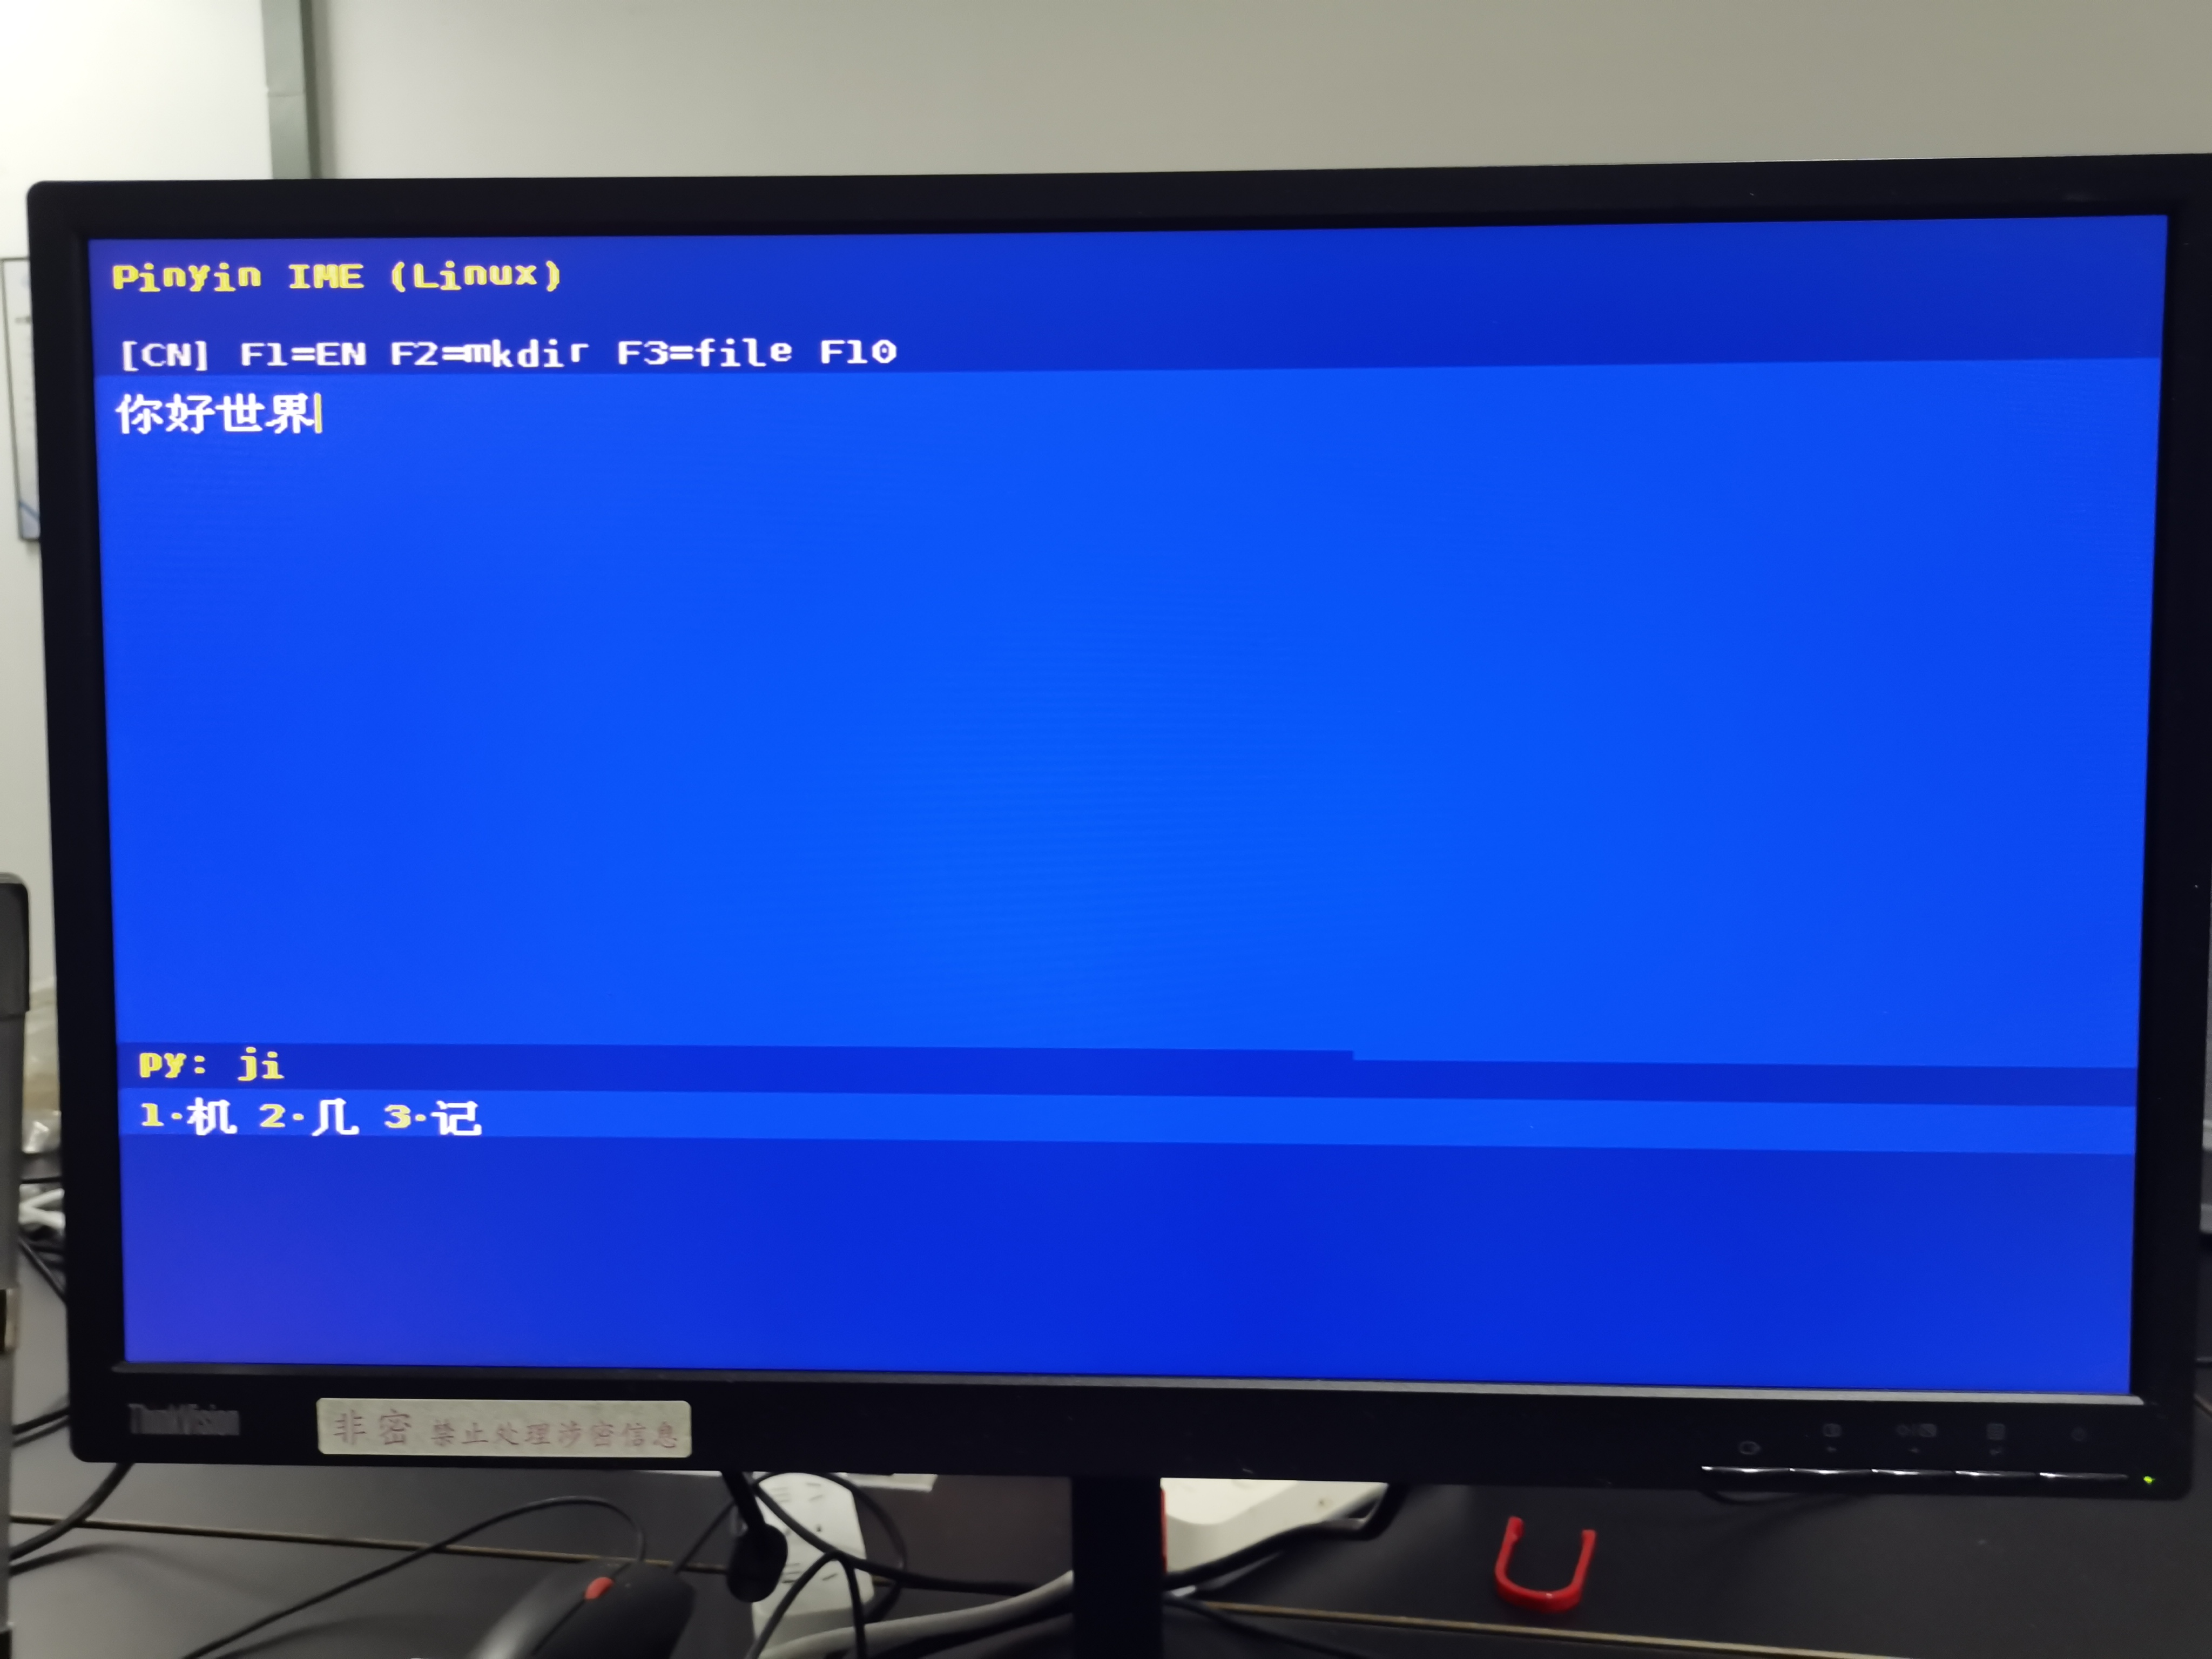
\includegraphics[width=0.95\textwidth]{figure/中文输入法.jpg}
  \caption{中文输入法}
  \label{fig:中文输入法}
\end{figure}

\begin{figure}[H]
  \centering
  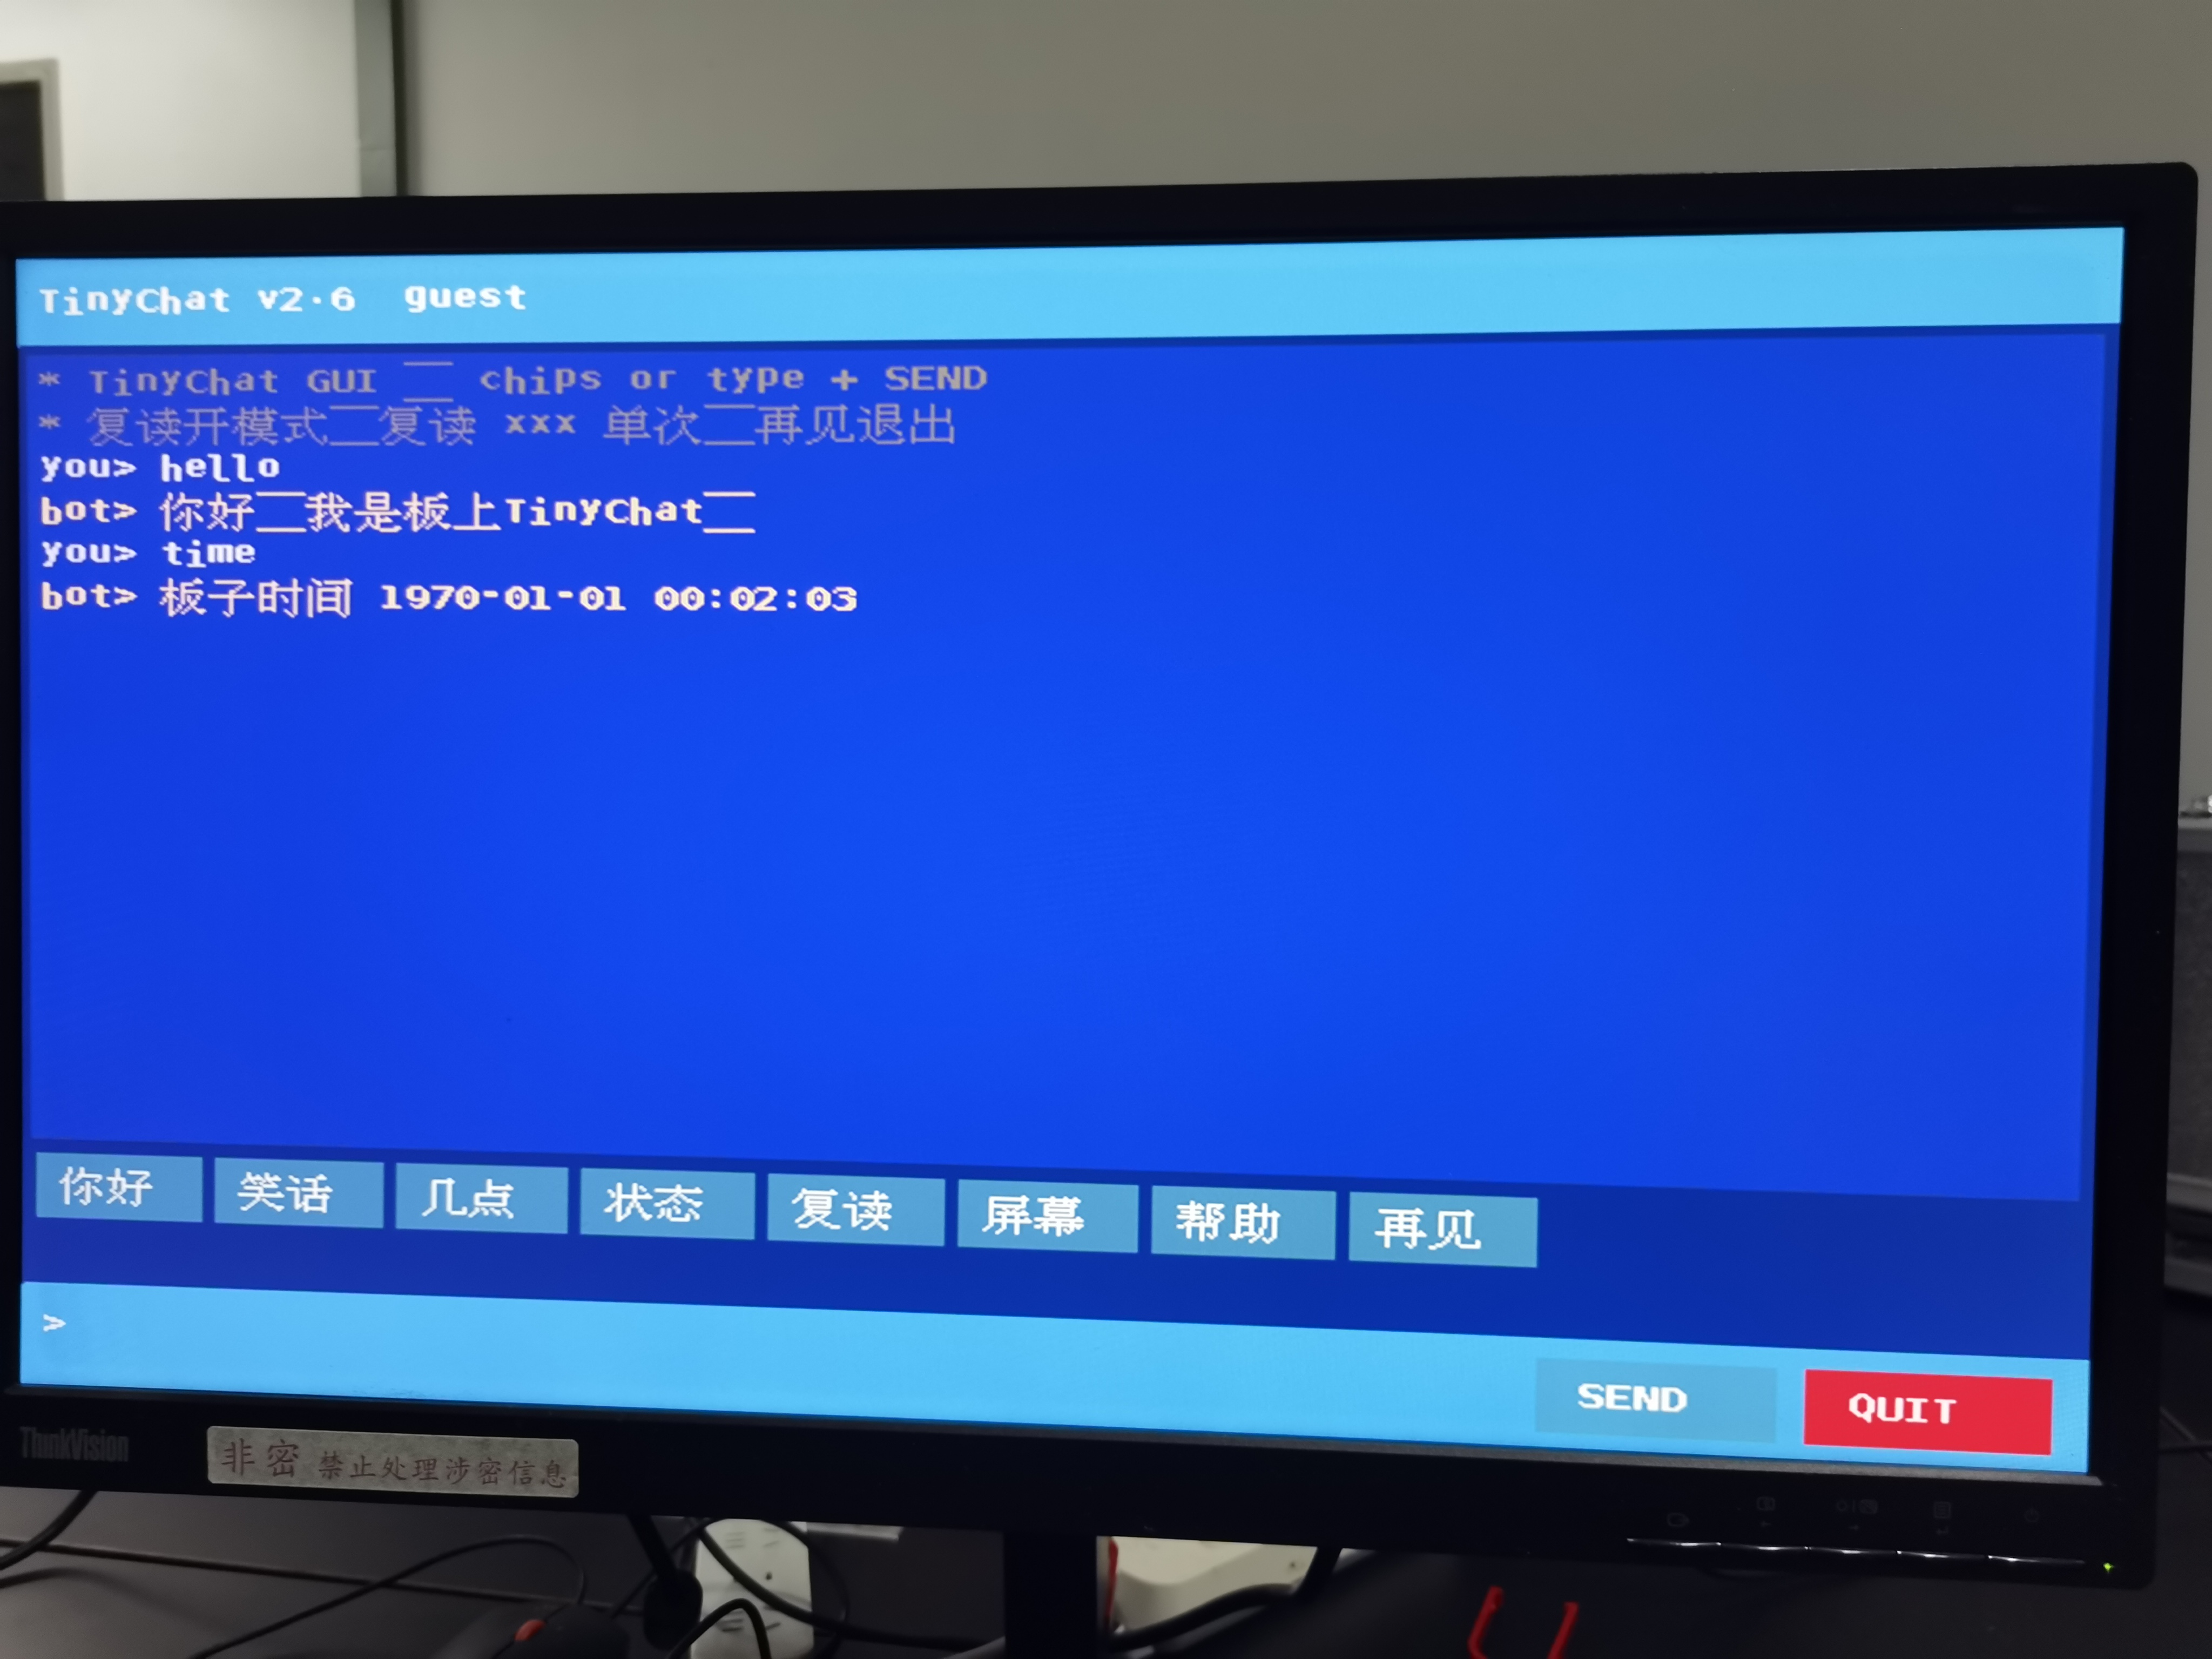
\includegraphics[width=0.95\textwidth]{figure/小AI对话.jpg}
  \caption{小AI对话}
  \label{fig:小AI对话}
\end{figure}

\begin{figure}[H]
  \centering
  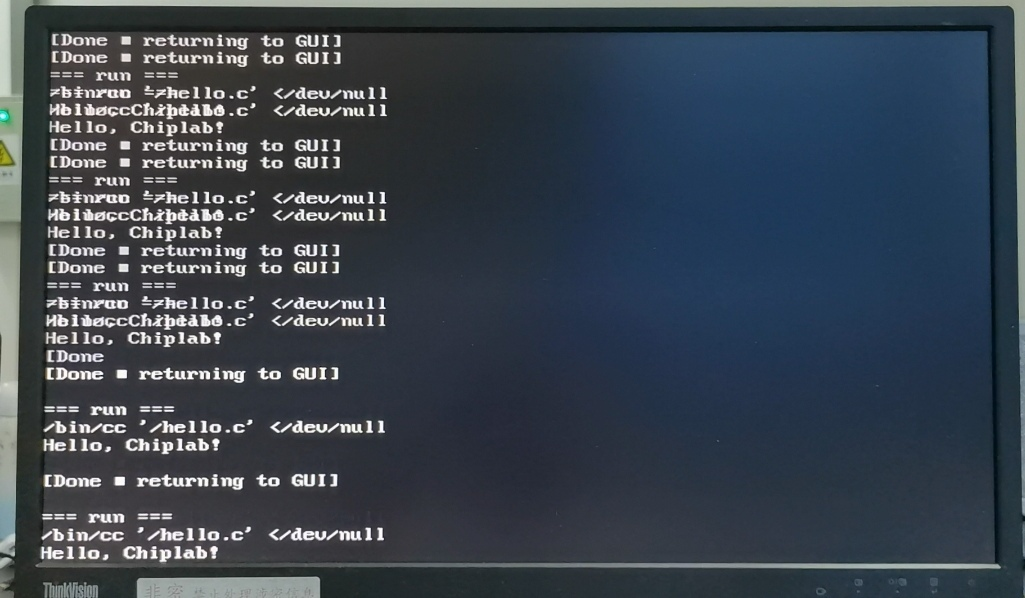
\includegraphics[width=0.95\textwidth]{figure/文件管理系统_执行代码.jpg}
  \caption{执行代码}
  \label{fig:执行代码}
\end{figure}

\begin{figure}[H]
  \centering
  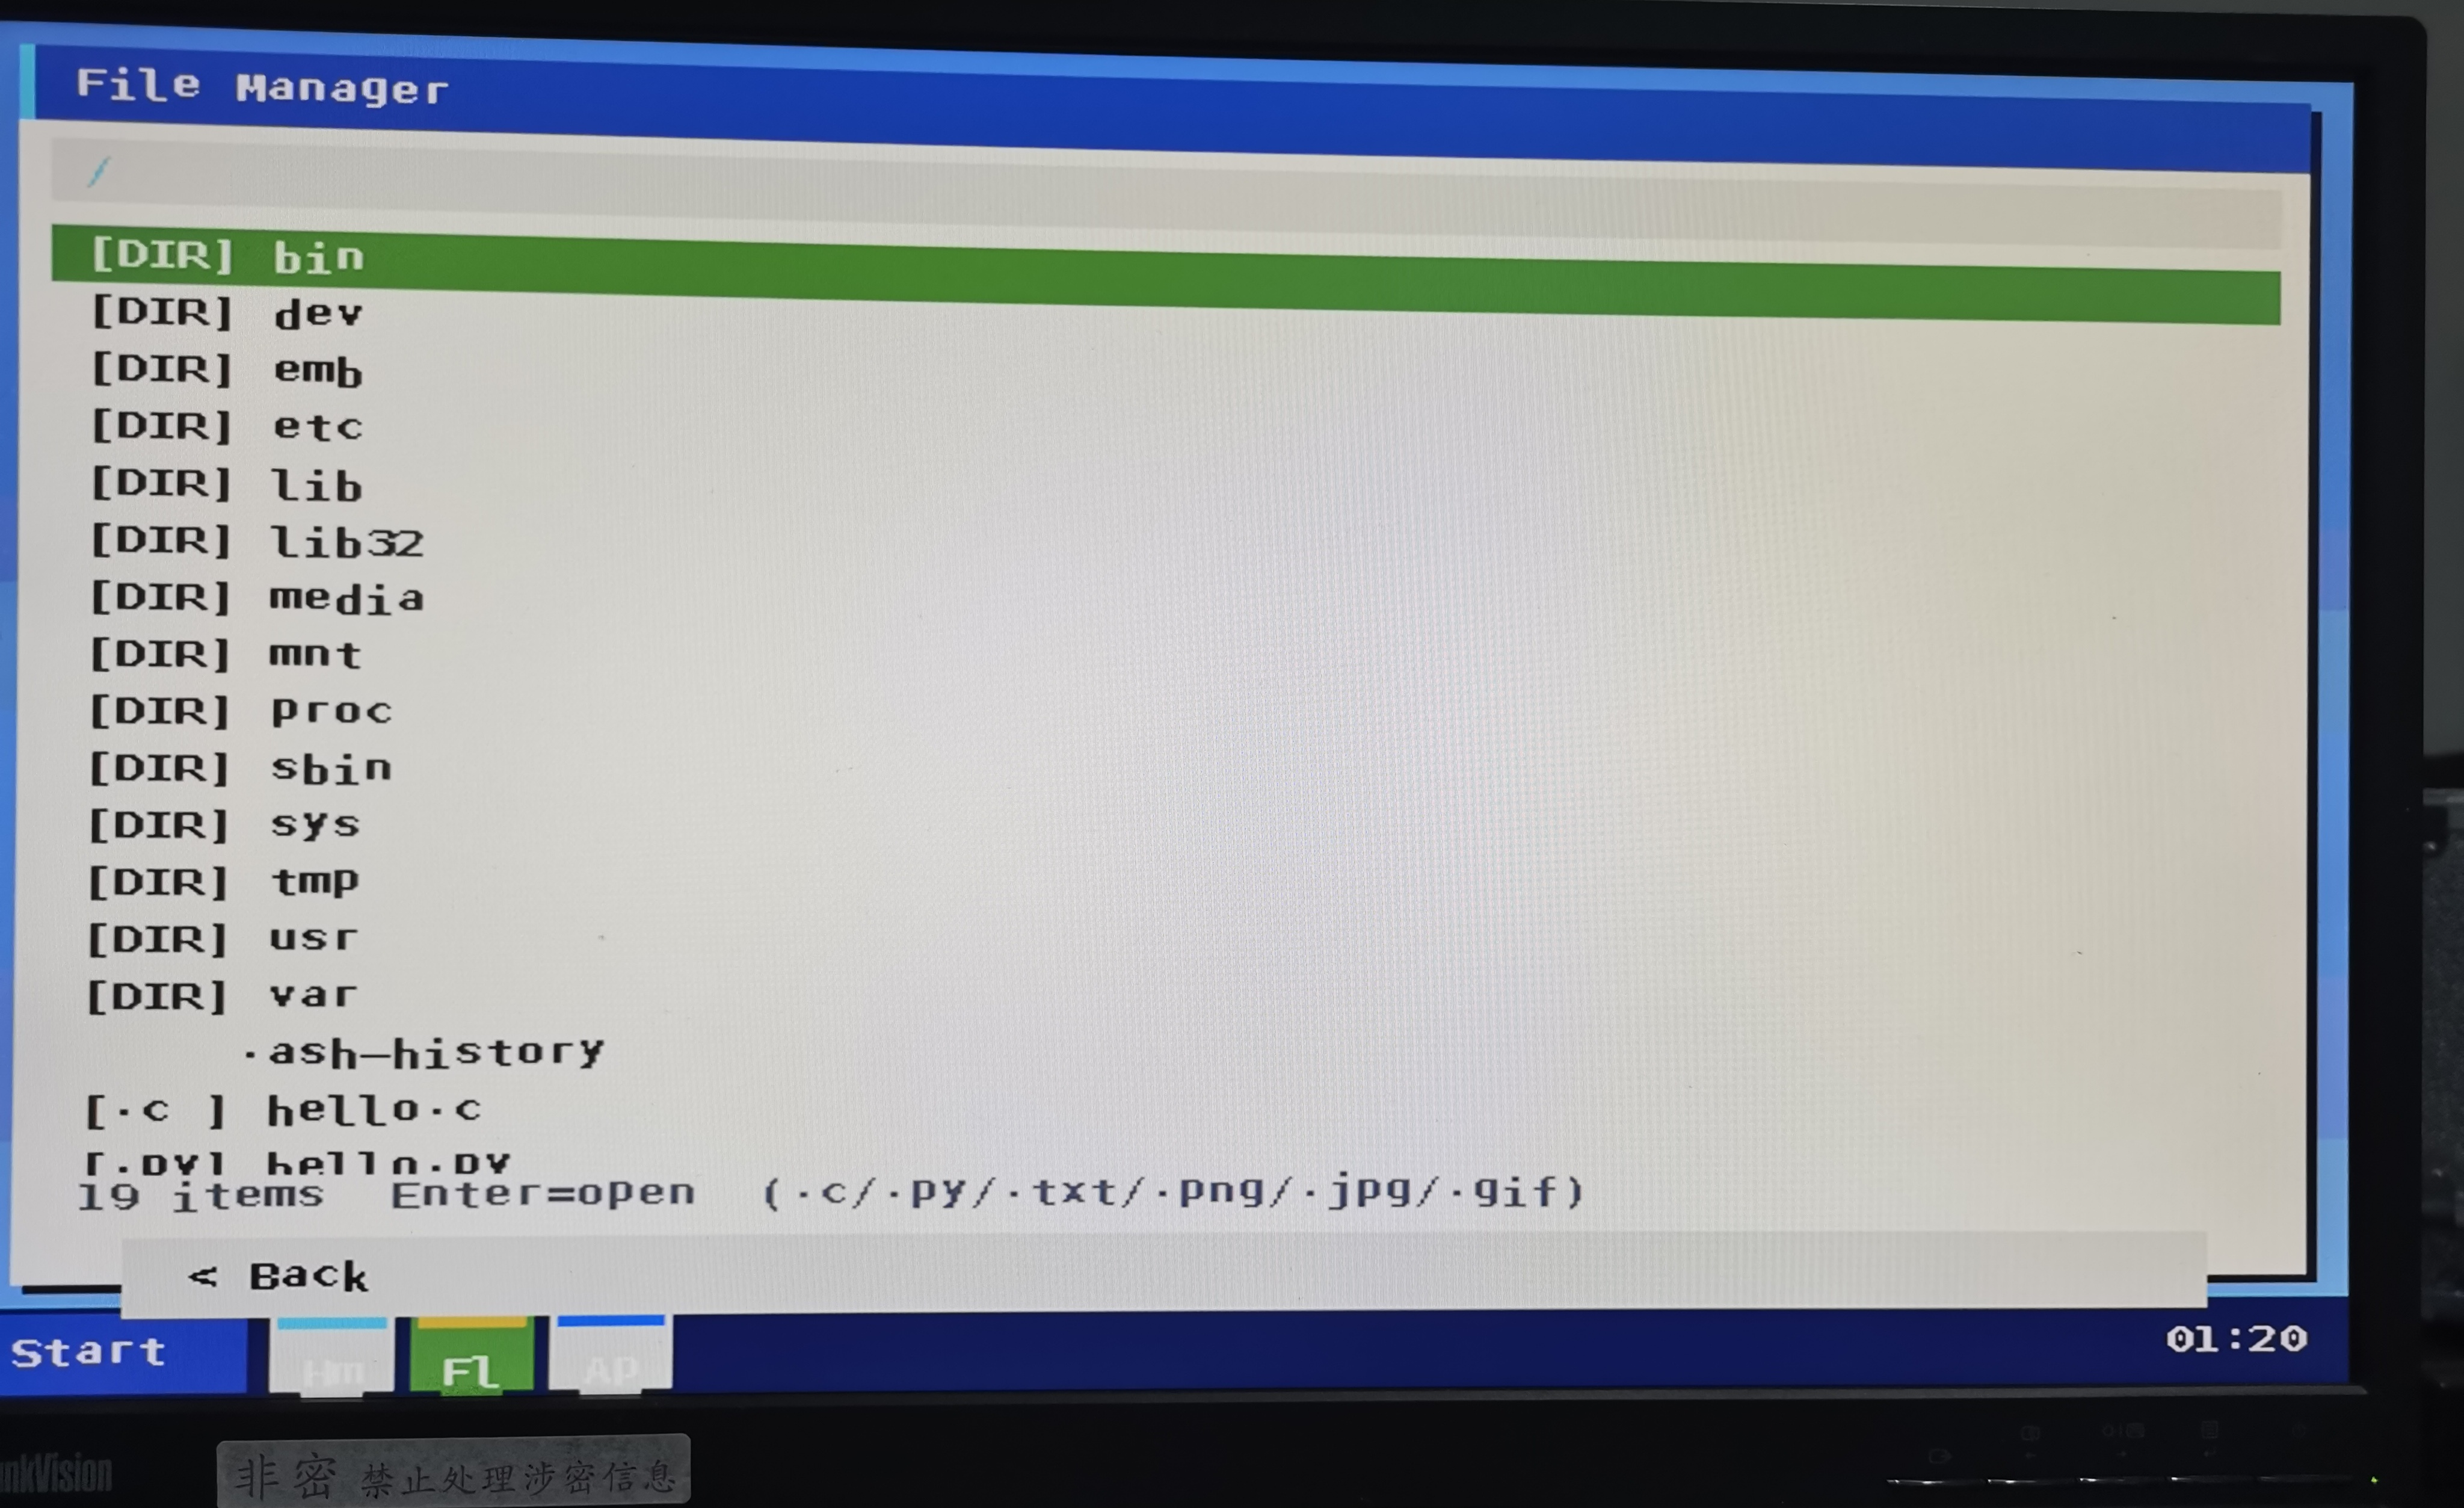
\includegraphics[width=0.95\textwidth]{figure/文件管理系统.jpg}
  \caption{文件管理系统}
  \label{fig:文件管理系统}
\end{figure}

\begin{figure}[H]
  \centering
  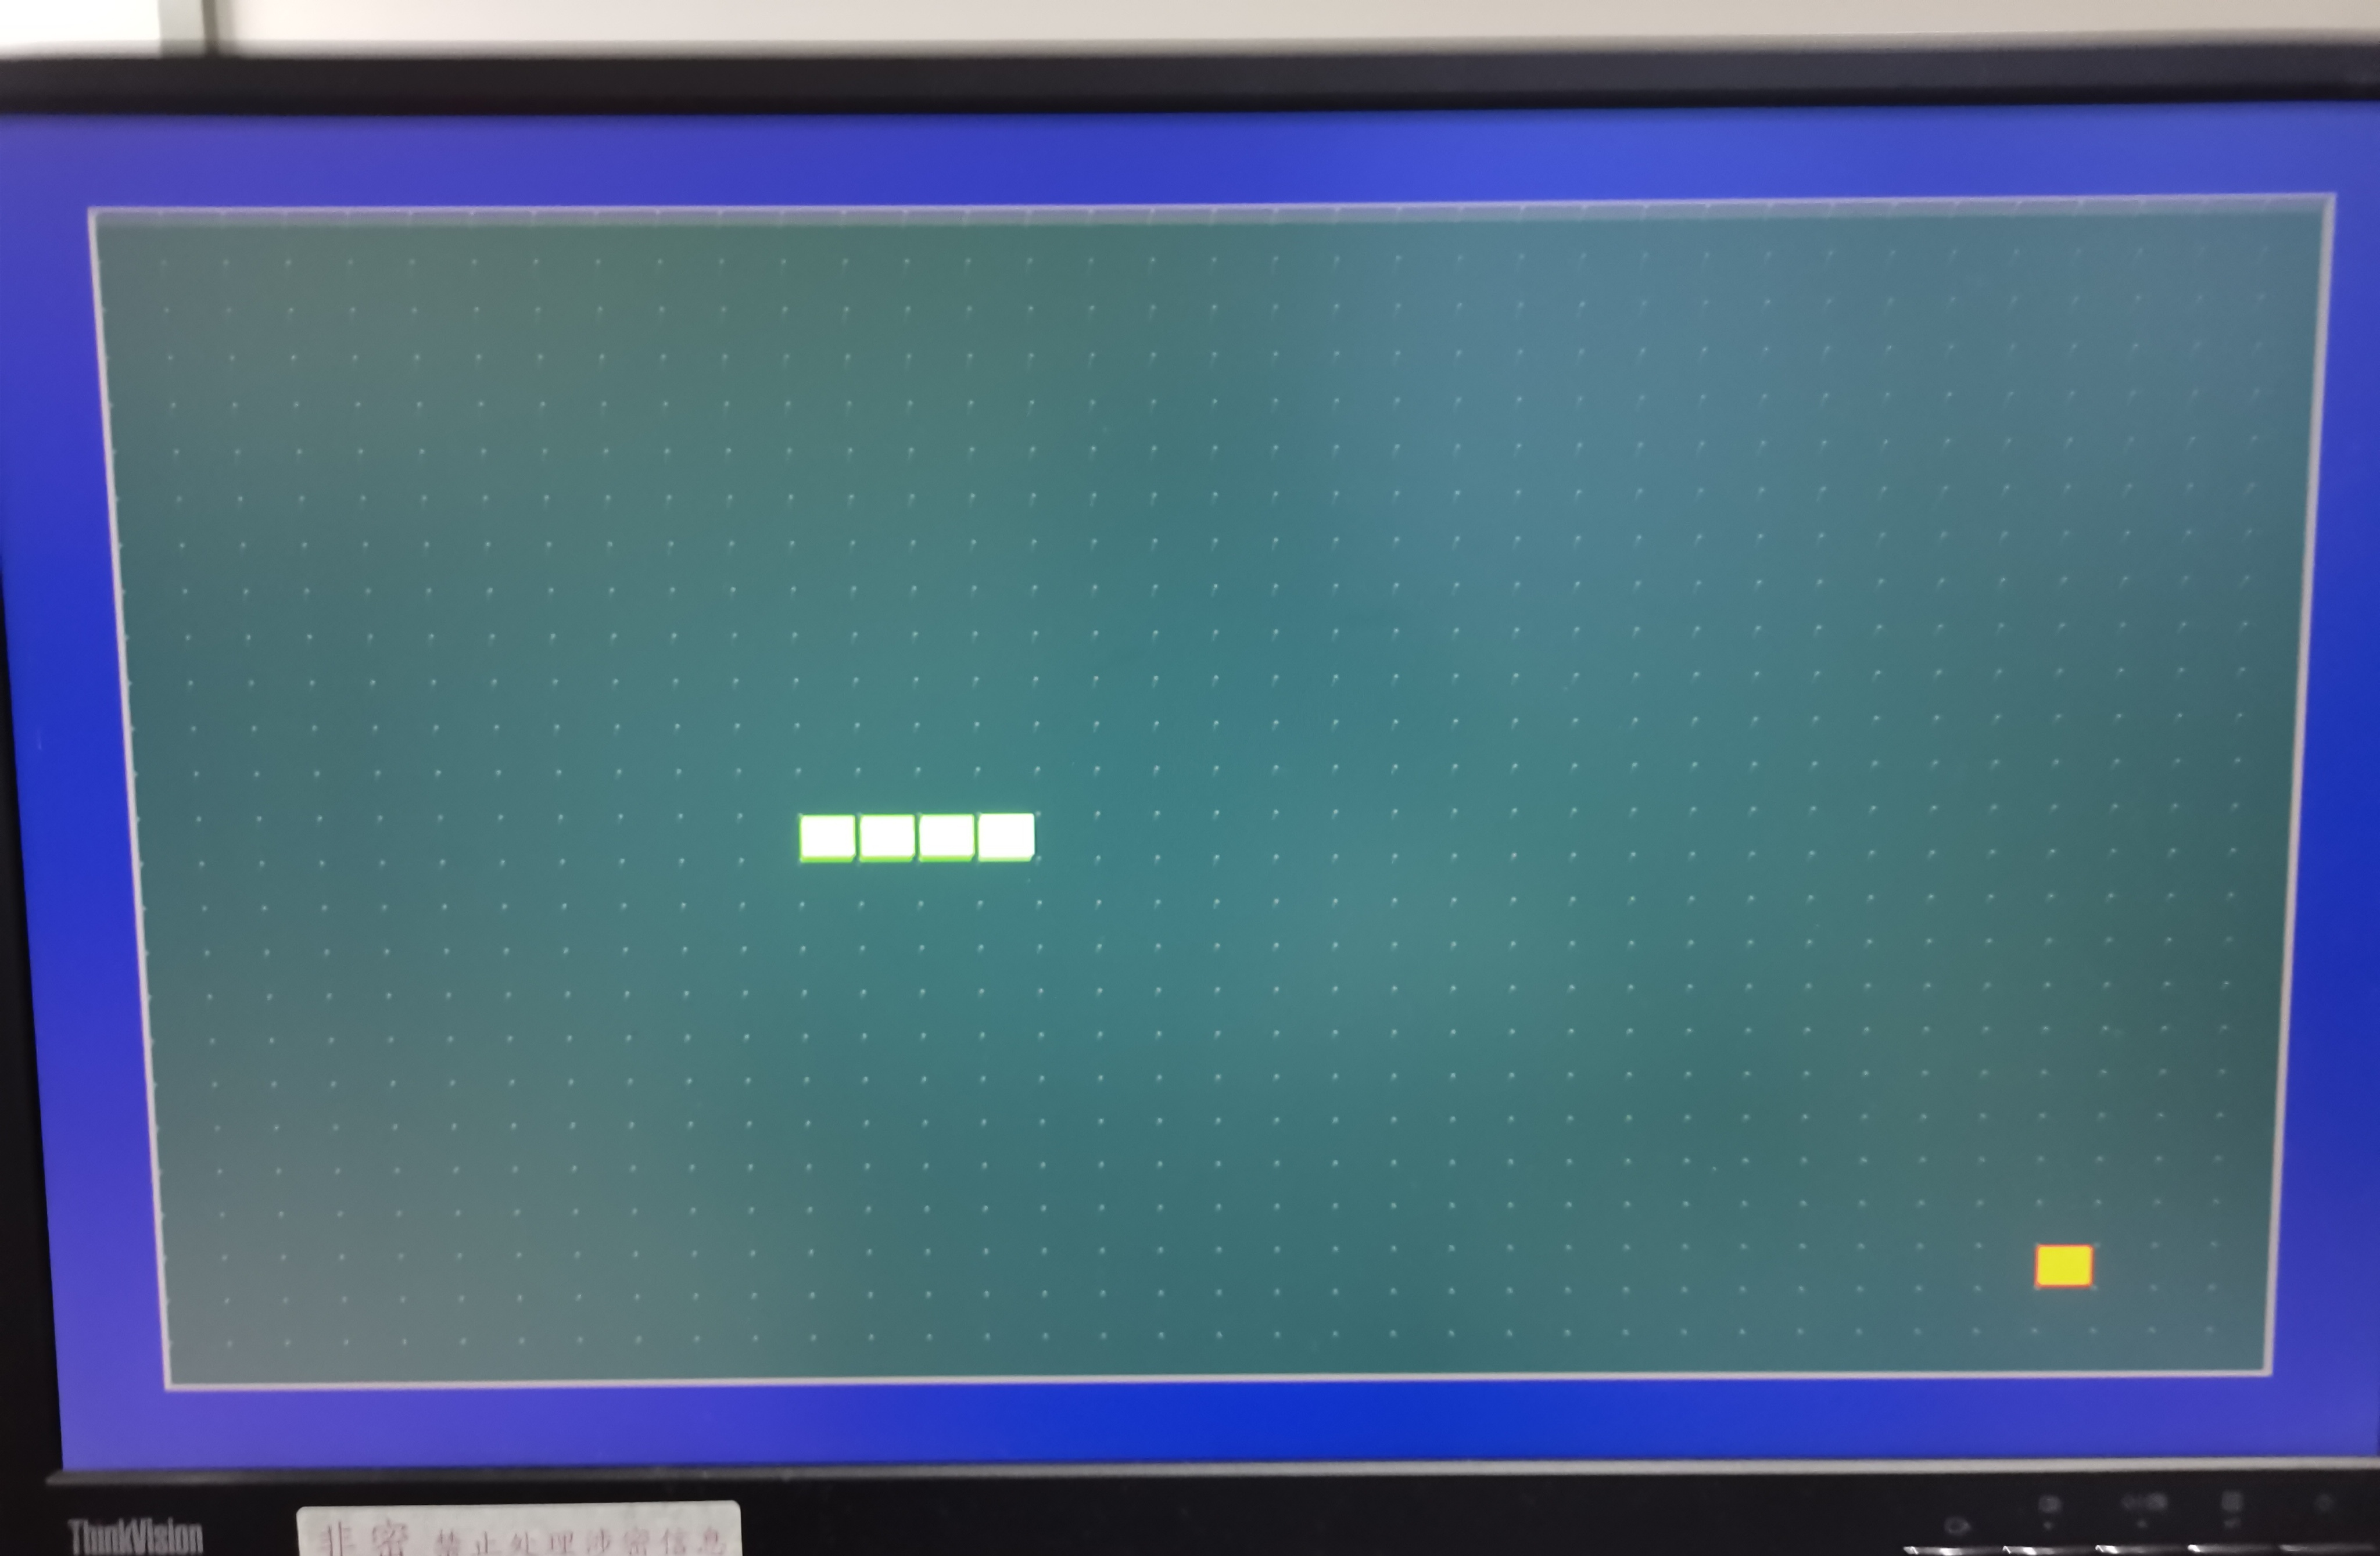
\includegraphics[width=0.95\textwidth]{figure/贪吃蛇.jpg}
  \caption{贪吃蛇}
  \label{fig:贪吃蛇}
\end{figure}

\begin{figure}[H]
  \centering
  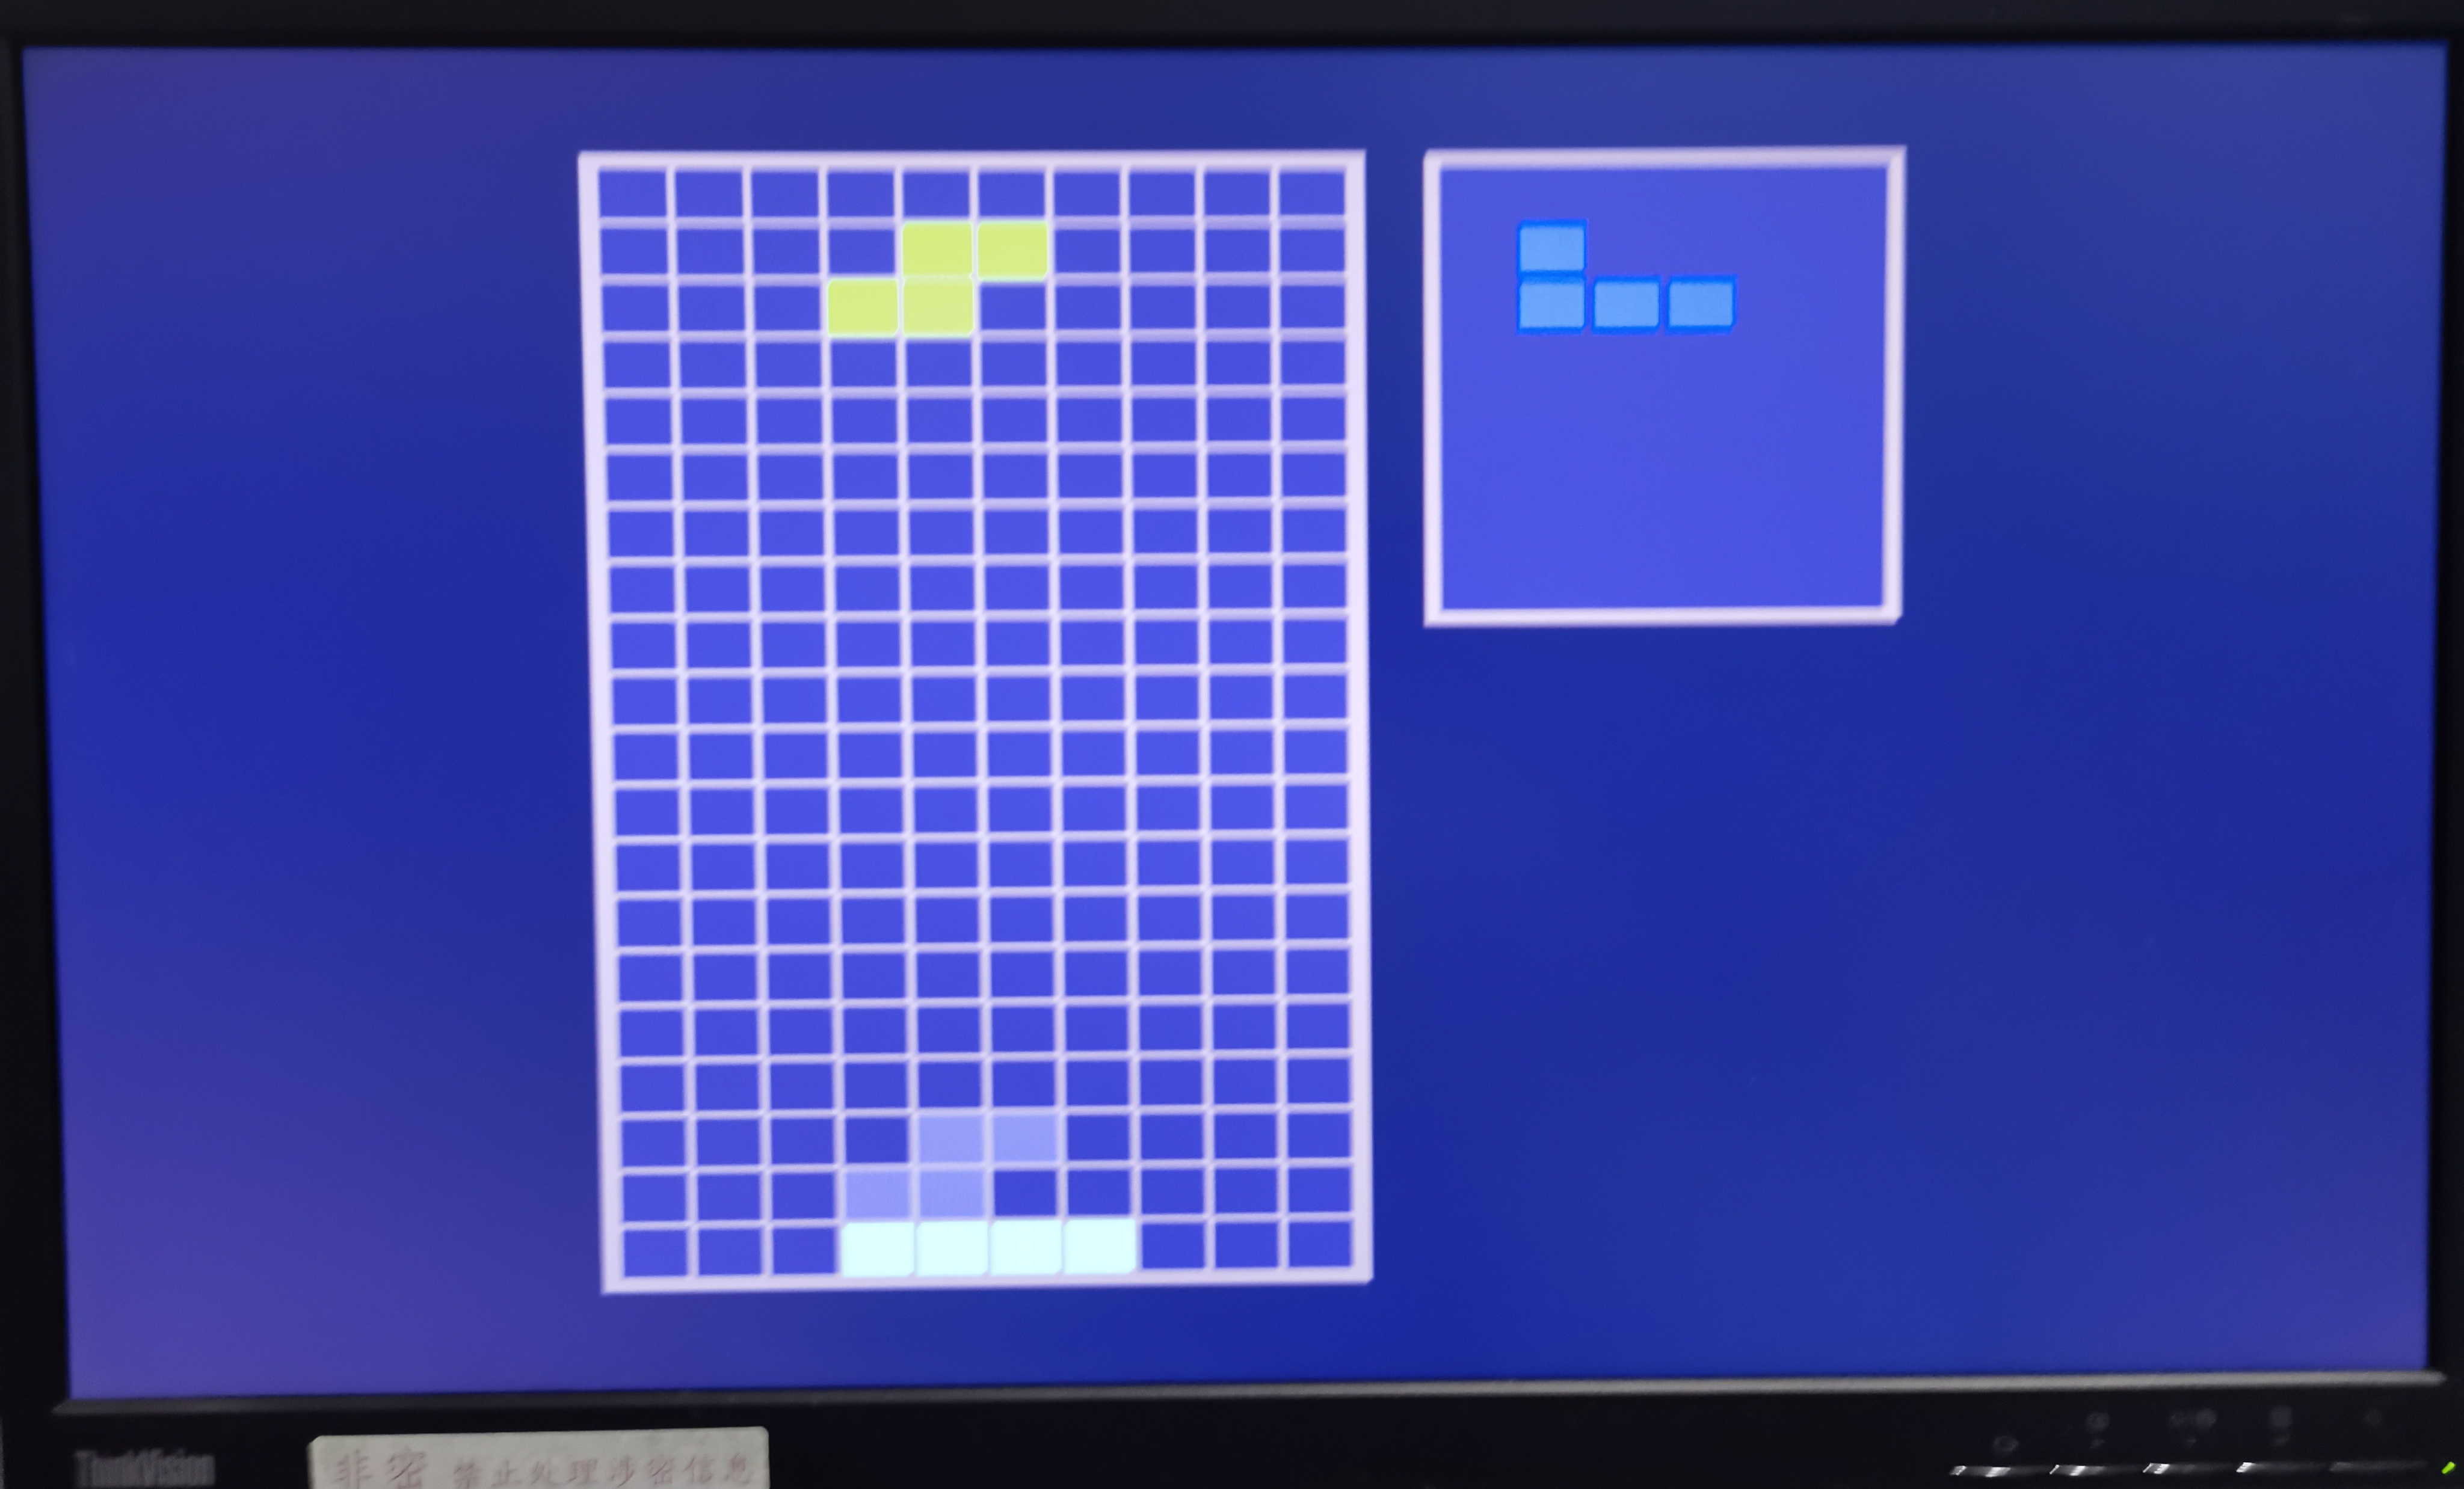
\includegraphics[width=0.95\textwidth]{figure/俄罗斯方块.jpg}
  \caption{俄罗斯方块}
  \label{fig:俄罗斯方块}
\end{figure}

\begin{figure}[H]
  \centering
  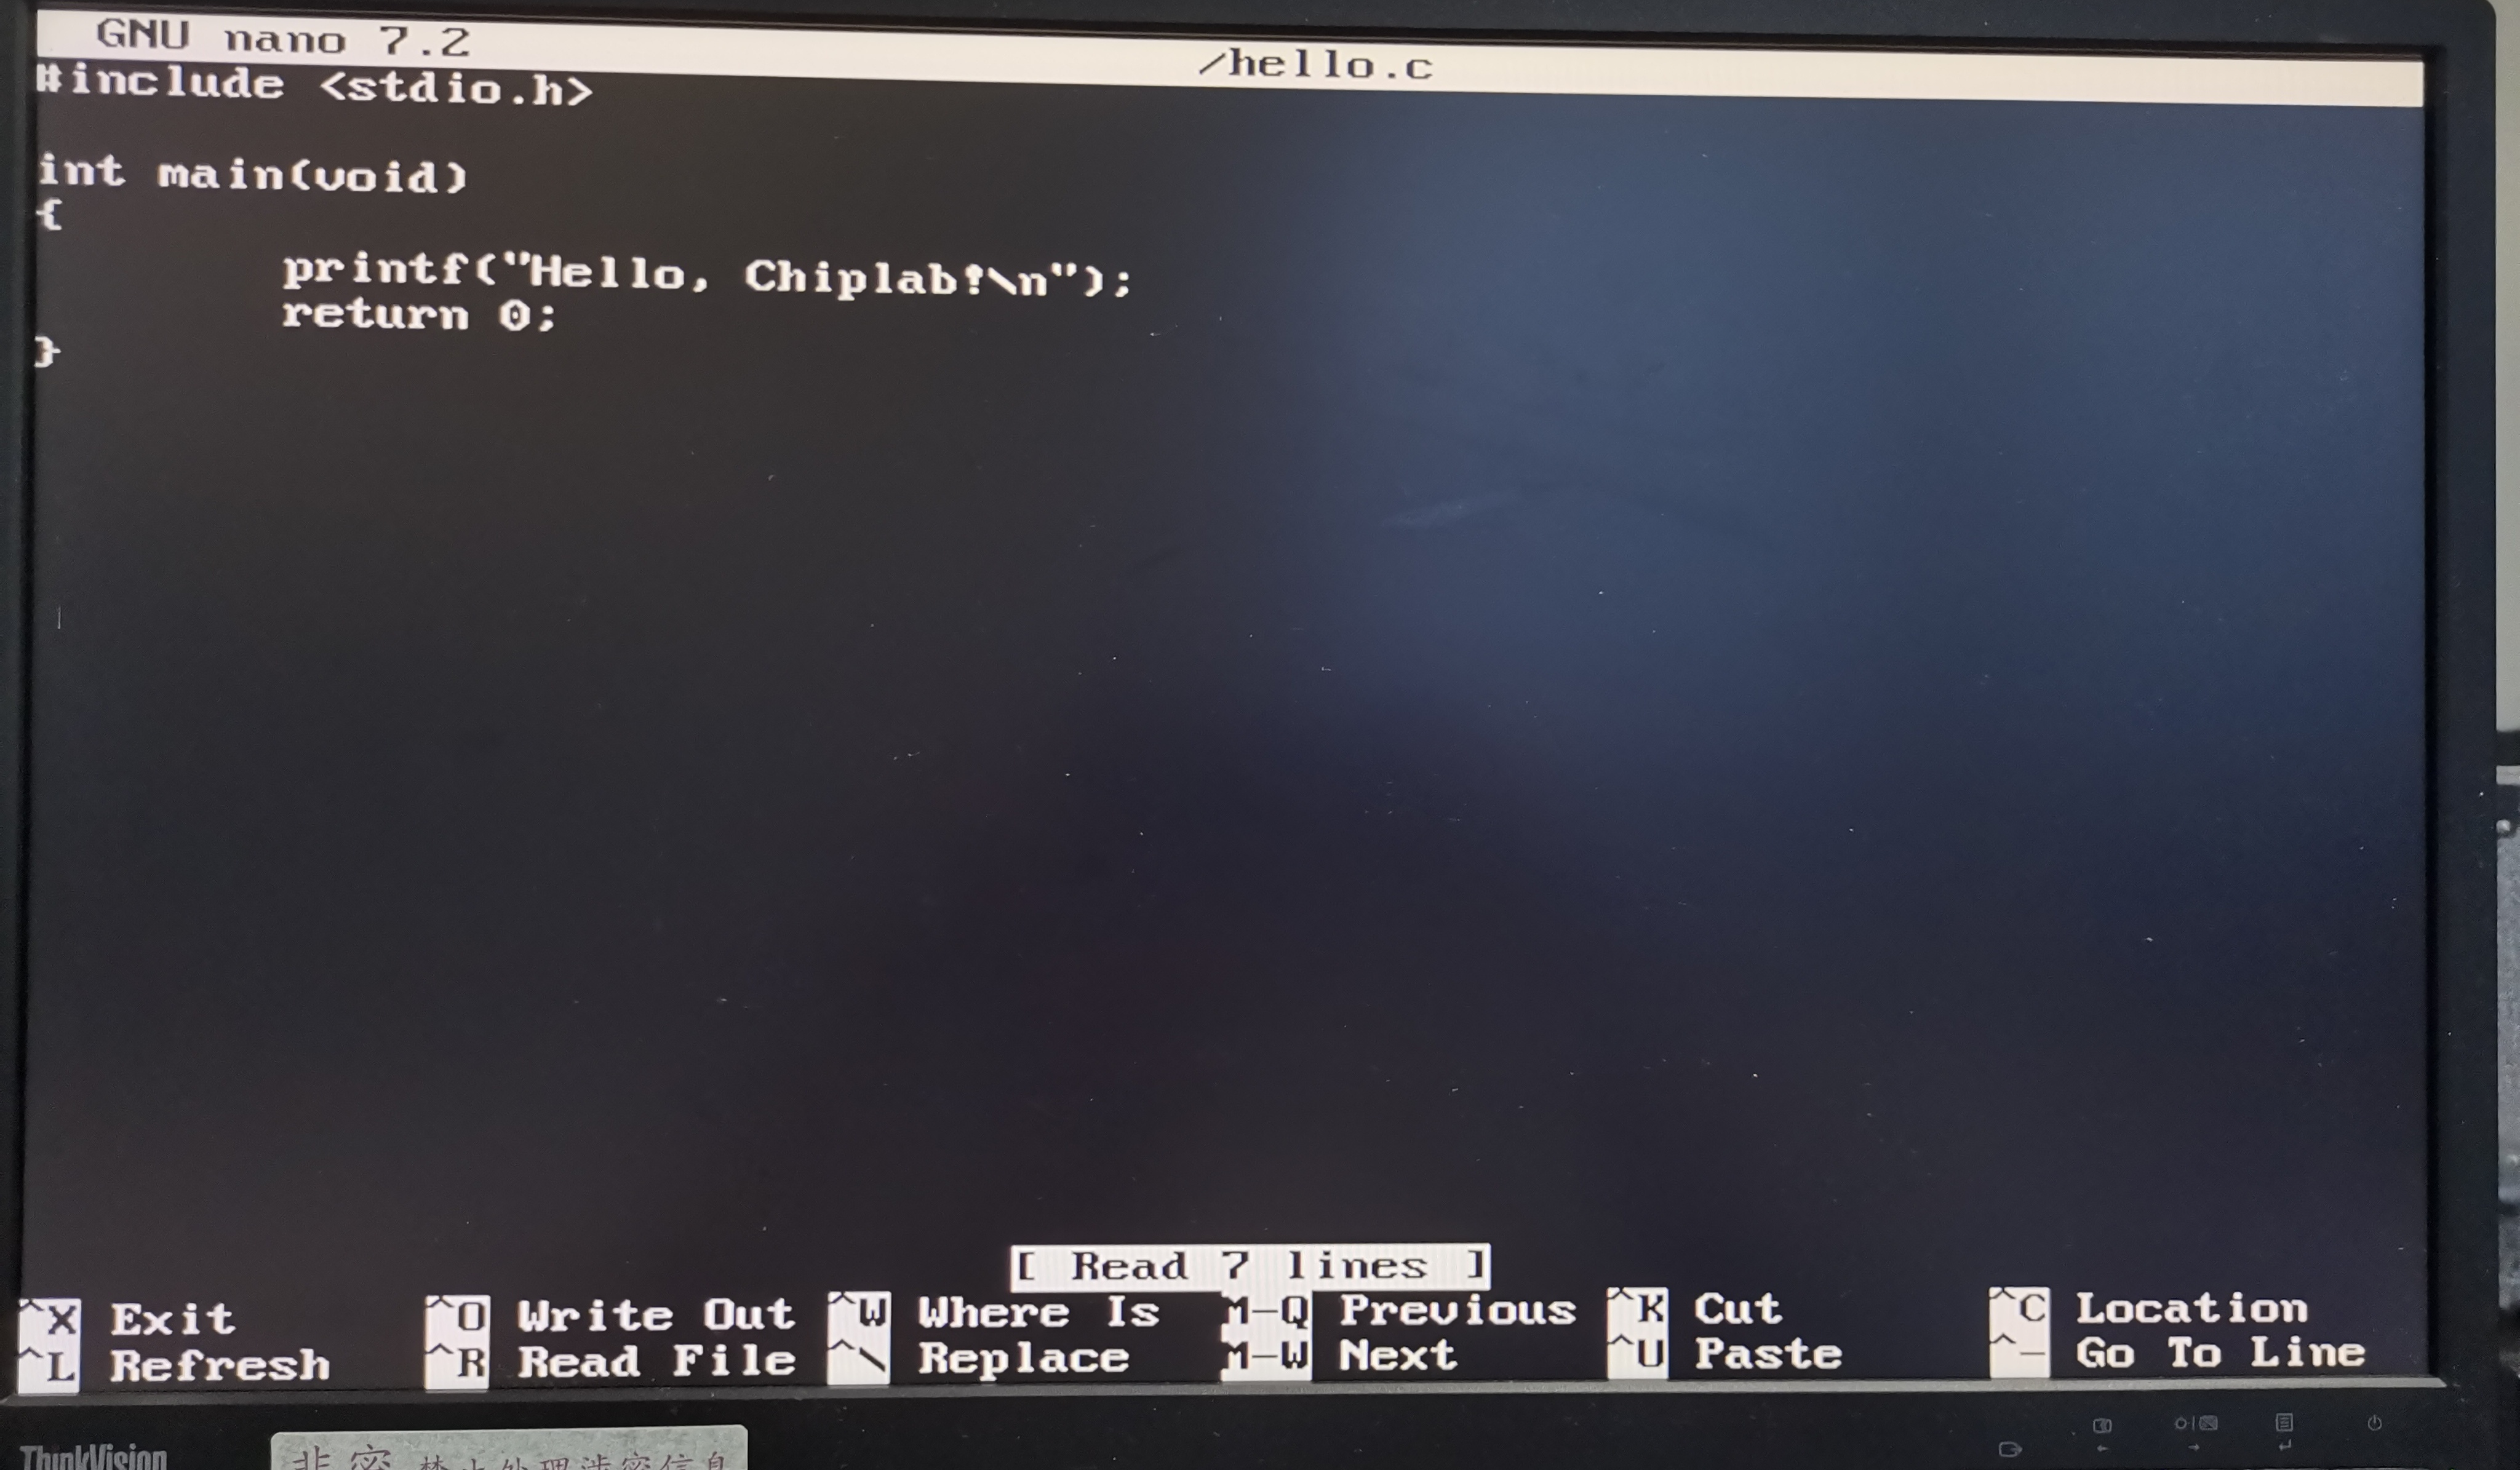
\includegraphics[width=0.95\textwidth]{figure/NANO.jpg}
  \caption{NANO}
  \label{fig:NANO}
\end{figure}

\begin{figure}[H]
  \centering
  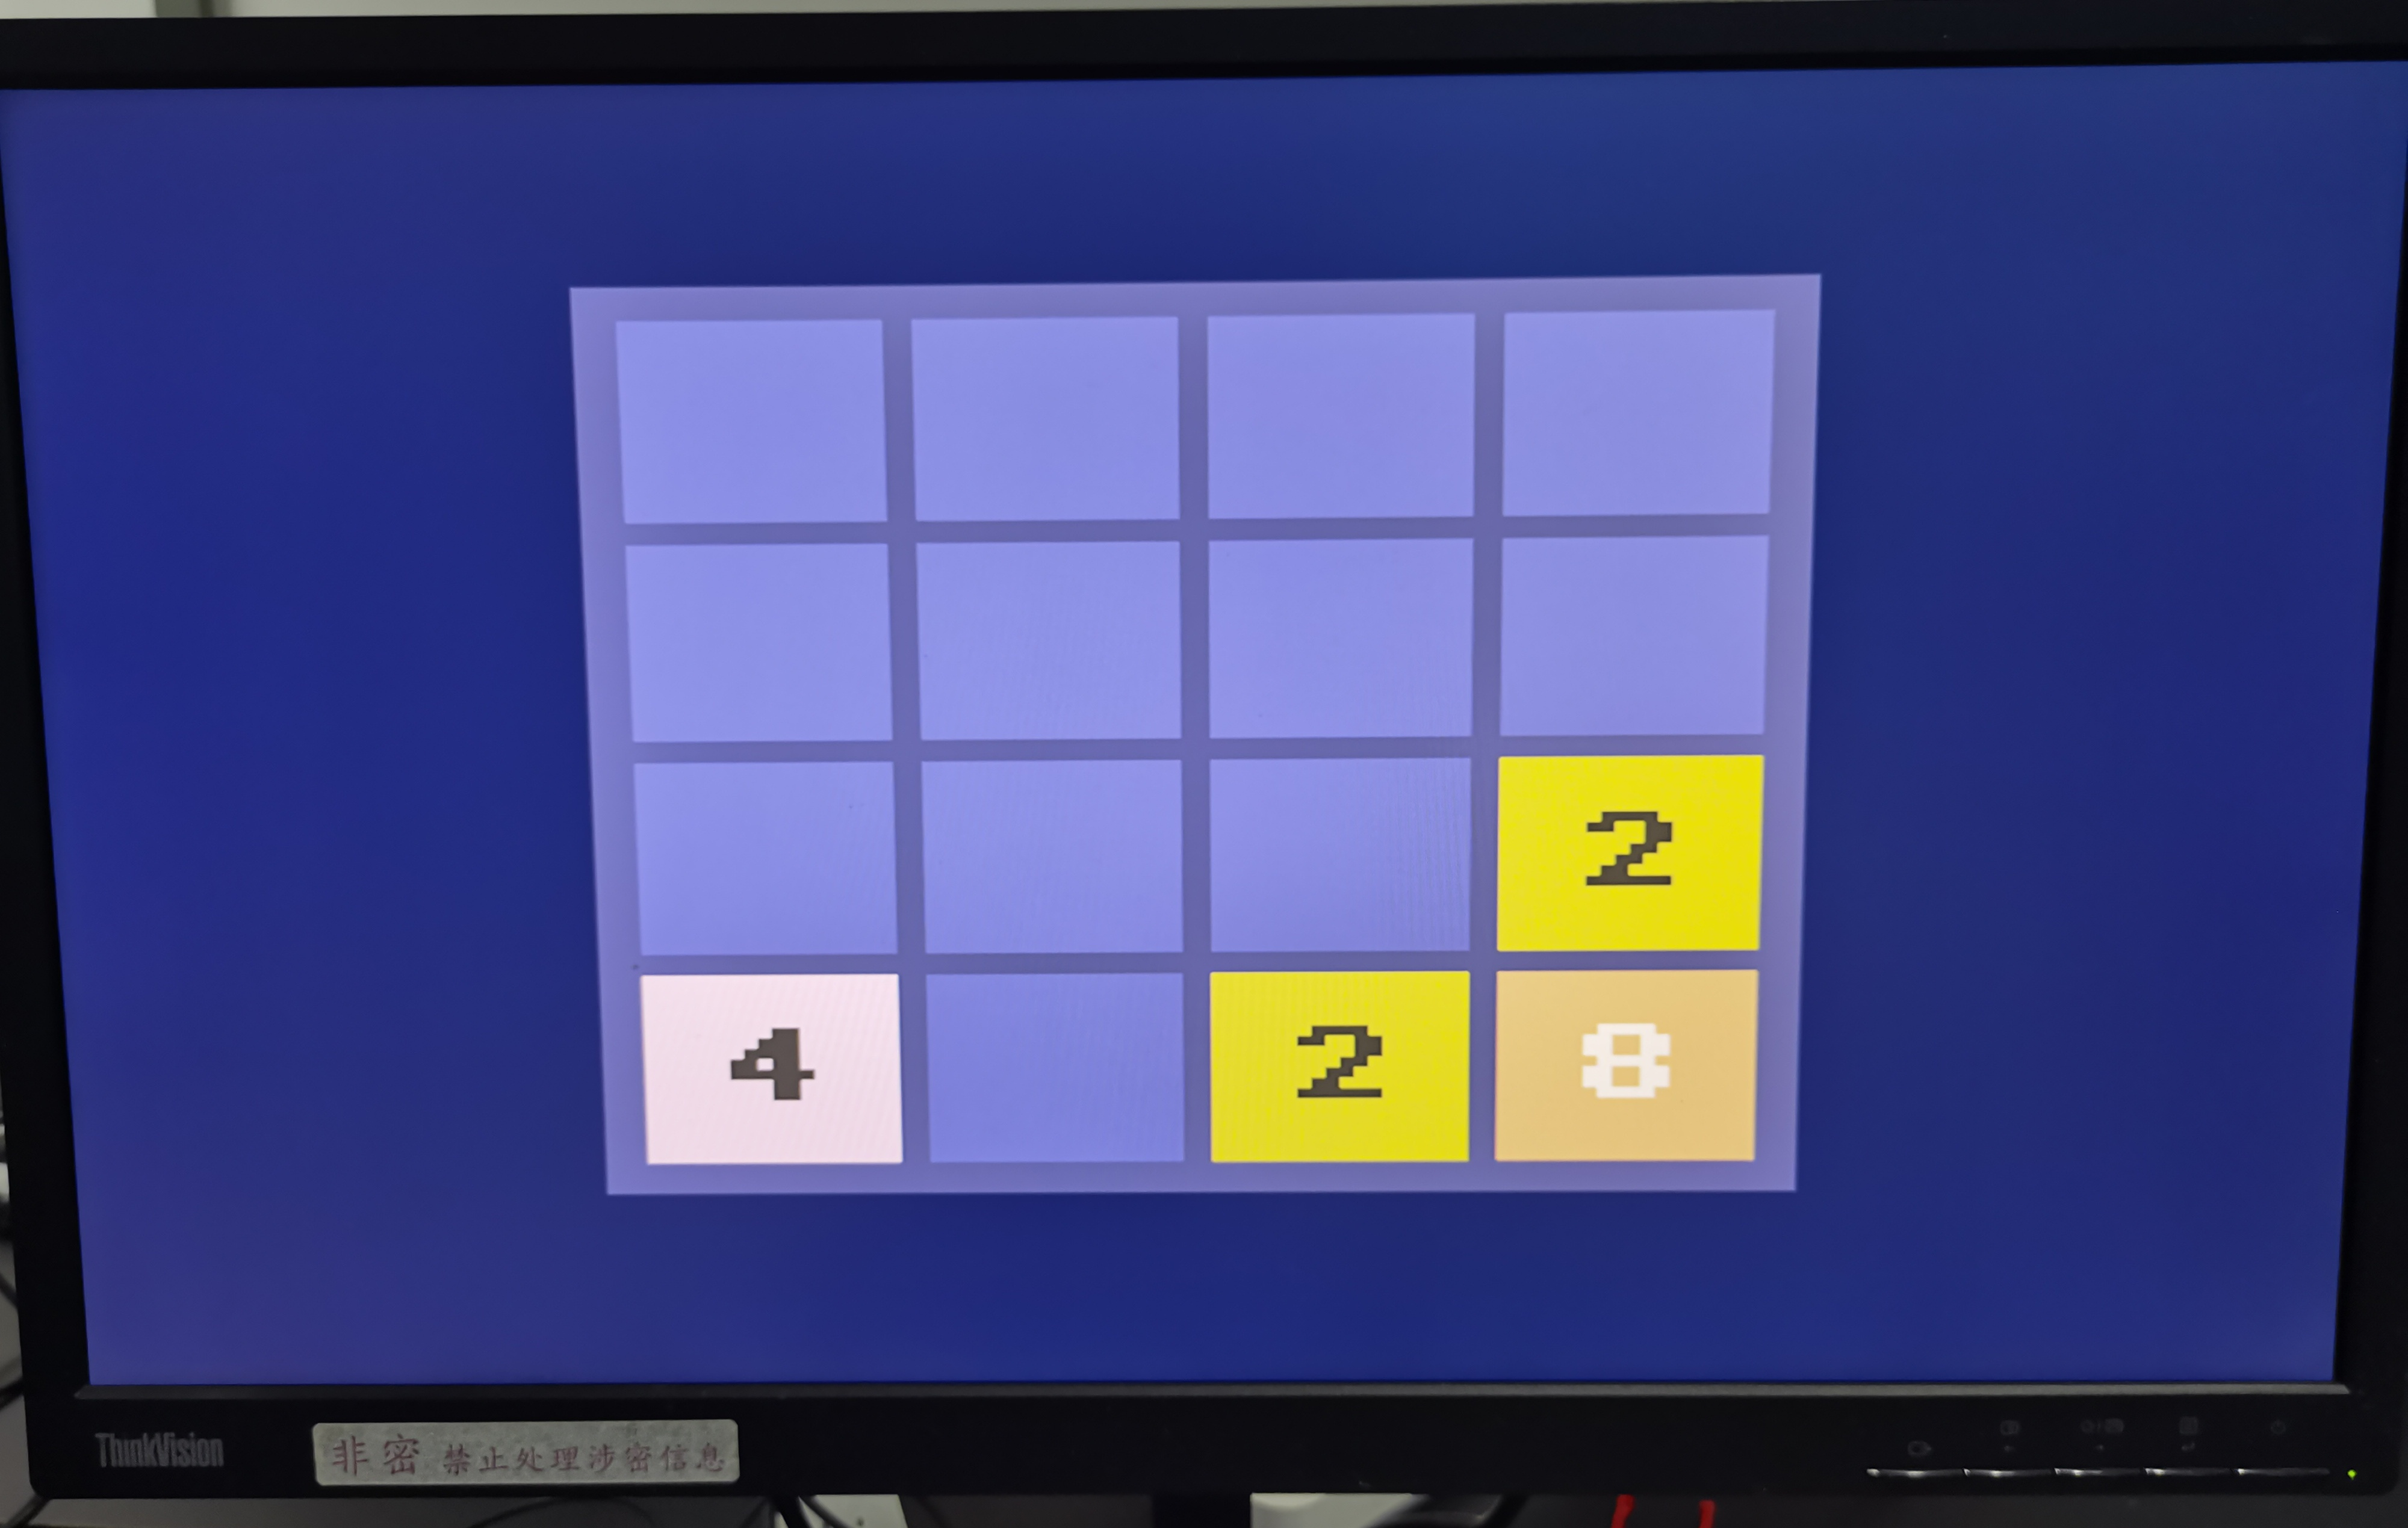
\includegraphics[width=0.95\textwidth]{figure/2048.jpg}
  \caption{2048}
  \label{fig:2048}
\end{figure}

\begin{figure}[H]
  \centering
  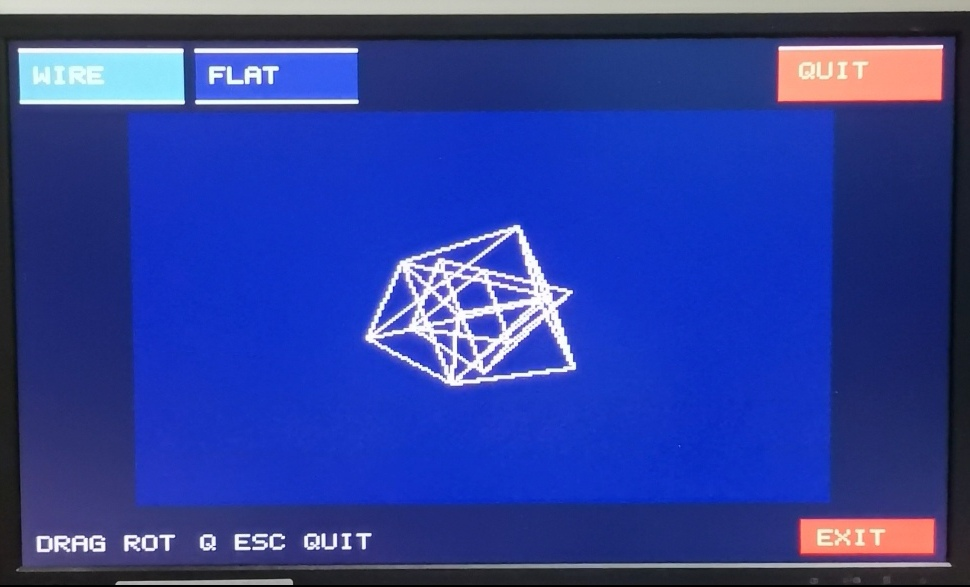
\includegraphics[width=0.95\textwidth]{figure/3D渲染_线条.jpg}
  \caption{3D渲染}
  \label{fig:3D渲染}
\end{figure}














